\documentclass{cslthse-msc}
\setcounter{tocdepth}{4}
\setcounter{secnumdepth}{4}
\usepackage[utf8]{inputenc}
\usepackage[english]{babel}
\usepackage{amsmath}
\usepackage{amsfonts}
\usepackage{amssymb}
\usepackage{amsthm}
%\usepackage{makeidx}
\usepackage{graphicx}
\usepackage[titletoc, header, page]{appendix}
\usepackage{todo}
\usepackage{float}
\usepackage[hidelinks]{hyperref}
\usepackage{wrapfig}
\usepackage[within=none]{caption}
\usepackage{pdfpages}
\usepackage{svg}
\usepackage{listings}
\usepackage{color}
\usepackage{tikz}
\usepackage{tikz-qtree}
\usetikzlibrary{trees}
\usepackage{capt-of}
\newcommand{\hilight}[1]{\colorbox{yellow}{#1}}

\definecolor{mygreen}{rgb}{0,0.6,0}
\definecolor{mygray}{rgb}{0.5,0.5,0.5}
\definecolor{mymauve}{rgb}{0.58,0,0.82}
\usepackage{colortbl}
  \definecolor{Lightgray}{RGB}{235,235,235}

\lstset{
breaklines=true,
language=SQL,
numbers=left,
numbersep=5pt,
numberstyle=\tiny\color{mygray},
frame=single,
basicstyle=\footnotesize,
captionpos=b
}
\newcommand{\bex}{BeX\textsuperscript{\textregistered}}
\renewcommand{\lstlistingname}{Algorithm}% Listing -> Algorithm
\renewcommand{\lstlistlistingname}{List of \lstlistingname s}% List of Listings -> List of Algorithms
\newcolumntype{H}{>{\setbox0=\hbox\bgroup}c<{\egroup}@{}}


\author{
	Alexander Söderberg \\
	{\normalsize \href{mailto:email@alexandersoderberg.com}{\texttt{email@alexandersoderberg.com}}}
	\and
	Max Åberg \\
    {\normalsize \href{mailto:aaberg.max@gmail.com}{\texttt{aaberg.max@gmail.com}}}
}

\title{Optimizing business intelligence
extraction speed from an
ERP-system’s database}
\subtitle{Master Thesis}
\company{Perfect IT BeX\textsuperscript{\textregistered} AB}
\supervisors{Lennart Söderberg, \href{mailto:lennart@perfectit.se}{\texttt{lennart@perfectit.se}}}{Alma Orucevic Alagic, \href{mailto:alma@cs.lth.se}{\texttt{alma@cs.lth.se}}}
\examiner{Per Andersson, \href{mailto:per.andersson@cs.lth.se}{\texttt{per.andersson@cs.lth.se}}}

\date{\today}

\acknowledgements{
\todo{Skriv acknowledgments}
}

\theabstract{
\todo {Skriv abstract}

}

\keywords{MSc, MsSQL, ERP, Optimization}

%% Only used to display font sizes
\makeatletter
\newcommand\thefontsize[1]{{#1 \f@size pt\par}}
\makeatother
%%%%%%%%%%


\begin{document}
\makefrontmatter

\chapter[Introduction]{Introduction}
2014 was the year of the cloud. Software companies strived to make their services cloud based in order to meet the increasing demands from the market of availability and reliability. 	
In today's businesses there's high demand for accurate and up-to-date business intelligence (henceforth referred to as BI). \todo{Not finished at all.}

\chapter{Background}\label{sec:background}

\section{Background}
Perfect It BeX AB was founded by Lennart Söderberg and Niklas Lindgren in 2007. In the beginning they made business extensions such as B2B, e-commerce and retail for the Microsoft Navision ERP. Eventually they started development of their own ERP-system to accommodate their extensions since they felt limited buy the technologies on which Navision was based. In 2010 they released three products; \bex Online, \bex Retail, and \bex B2B. \bex Online is the main product on which the other products rely. It is a completely cloud-based ERP-system specialized for the retail industry. The main functionality in \bex Online are:

\begin{itemize}
\item Financial tools
\item Sales administration \& handling
\item Purchase handling
\item Inventory and Warehousing
\item History and Business Reports
\end{itemize}

In recent years, Perfect It has felt an increasing demand from customers for better business intelligence capabilities. In response to this they have improved the Business Report functionality in \bex Online, to be able to give a wider range of different financial key values. According to Lennart, being able to offer their customers tools enabling for good business intelligence, is key to staying competitive. Therefore, they want to develop these tools further to make them better and to include more functionality. However, they have noticed that generating some of the reports can take a relatively long time, especially for their bigger clients whose system's have a lot of data.

\subsection{BI-reports}\label{sec:BI}
see Figure \ref{fig:BI} in Appendix \ref{sec:appTabIll}

\begin{itemize}
\item What are they used for?
\item How are they done?
\item Where are they?
\item Which of them are used most and/or are critical for the system?
\end{itemize}

\section{Problem description}
Perfect It \bex AB was motivated to collaborate with academia in order to investigate how to increase the generation speed of the business intelligence-reports and to find a possible solution that increases this speed.

\section{Thesis Goals} \label{sec:goals}
The goal of this thesis is to identify issues related to the problem, and to propose a solution for speeding up the generation of BI reports in Perfect IT \bex AB's product \bex Online. To be able to speed up the BI report generation the processes responsible needs to be analyzed and optimized or rebuilt for speed. The solution needs to be versatile to handle the current system, to handle new functionality and also future company growth. Hence, the suggested changes needs to be scalable. Taking in to account that Perfect IT \bex has one physical server, the scalability should be vertically\cite{scalability} since the company will provide the system to more clients in the future.\\\\
In order to make the above optimization possible, the following goals have been established:
\begin{enumerate}
\item Identify the most common causes to db inefficiency.
\item The current processes behind generation of the BI-reports must be identified and mapped in order to identify bottle-necks and inefficiencies.
\item The academic approach should be done as a "Problem Solving Research"-process and will propose \& test a possible solution.
\item Analyze possible solutions to decide which of them are a best fit for the case company.
\item Implement the solutions in \bex Online and perform a final analysis to determine if the case company's goal was met.
\end{enumerate}
  
\section{Scope} \label{sec:scope}
\hilight{According to Nevarez\cite{Nevarez} the main areas of investigation while trying to optimize an existing database for speed are:}
Because of the problems and goals described in the background the focus should be on the following main areas of investigation:
\begin{itemize}
\item Query tuning
\item Execution plan tuning
\item Index tuning
\item Database execution statistics
\item In-Memory OLTP
\item Plan caching
\end{itemize}
Due to the limited time frame of this thesis, all of these areas won't be explored. With respect to this and the company's preferences the following focus areas were decided upon: Query tuning, index tuning and "In-Memory OLTP"-solutions.

\section{Limitations}

The objective is primarily to increase the speed of the ERP-system's business intelligence reporting module by optimizing the database. The database is used by all parts of \bex Online. This means that the following limitations to the developed solution must be in place.

\begin{itemize}
\item The solution must not affect any functionality in \bex Online.
\item The solution must not decrease performance in other \bex Online functionality.
\item The solution must work with the current implementation of \bex Online Back-end.
\end{itemize}

\section{Related Work}


\section{Contributions}

\chapter{Research Questions \& Methodology}

\section{Research Questions}
The research questions of this thesis were formulated in relation to the thesis goals in section \ref{sec:goals} and the scope in section \ref{sec:scope}. The thesis is formed to explain and answer the following research questions:
\begin{itemize}
\item	How does the current system function and what are the bottle-necks?
\item 	What are the most common approaches for improving database performance, with regard to index fragmentation, query tuning and In-memory-solutions?
\item	What optimization solutions are best-fit for the case company with regards to the goals, scope and limitations?	
\item	How can the proposed solution be implemented in Perfect IT \bex AB's current system?
\end{itemize}

\section{Methodology}
This thesis is of a problem solving nature and should continuously adapt to changing conditions. The methodology used should therefore preferably be flexible. A methodology that provides valuable support and is intended to improve something while studying it is action research \cite{robson}. Action research begins with an observation phase that identifies and clarifies the problems that are present, for this thesis that is presented in chapter \ref{sec:background}. In chapter \ref{sec:proposedsoluton} the next step in action research is stated, a proposed solution to the problem(s).\\

After implementing the proposed solution the next phase is the evaluation. The evaluation is made to verify the implementation in its context, to analyze and reflect on how it works in its integration. The whole action research is an iterative process and is based on the evaluation. Accordingly to Höst et. al. \cite{regnell} an evaluation is hard to keep unbiased, since the ones doing the critical evaluation are also the ones that performed the research. To counter an unbiased evaluation, some evaluation criteria were established based on the above mentioned goals in section \ref{sec:goals}. To ensure that all of the stakeholders goals are met this thesis will on a regular basis be reviewed both by supervisors at Perfect IT and at LTH.

\section{Work}
First of all an acquaintance of Perfect IT \bex AB's system needed to be established. In conjunction with the examination of the current system and its parts a literature research was performed. The area this research treats is extensively and the research done is almost indefinite. Therefore the literature research scope needed to be narrowed with its base in the currents systems examination.\\\\    
To find the literature and related work Engineering Village\cite{Enginvillage} and Google Scholar\cite{Googlescholar} together with DBLP\cite{DBLP} was used. A lot of time was dedicated to find relevant literature and information for this thesis and at the same time examine if the ideas established during the system examination phase were possible and solid solutions.\\\\
Using the paper written by Gruian and Lekebjer on formatting a master’s thesis\cite{Reportmall} and guidelines from the book by Höst et. al. \cite{regnell} the initial work on the master thesis report was conducted. 
\todo{to be continued\ldots}

\chapter{Approach}

\section{Technical System Description}
Perfect IT delivers web-based business systems and services specialized for the retail industry. The \bex Online ERP-system is distributed as a SaaS-solution and all clients share servers which makes it a true cloud based service. The clients access \bex Online's front-end through a web browser. \bex Retail and \bex B2B are connected directly to \bex Online's back-end.
The database for \bex Online is a Microsoft Server 2014 Web Edition.
\begin{figure}[H]
\vspace{-15pt}
  \begin{center}
    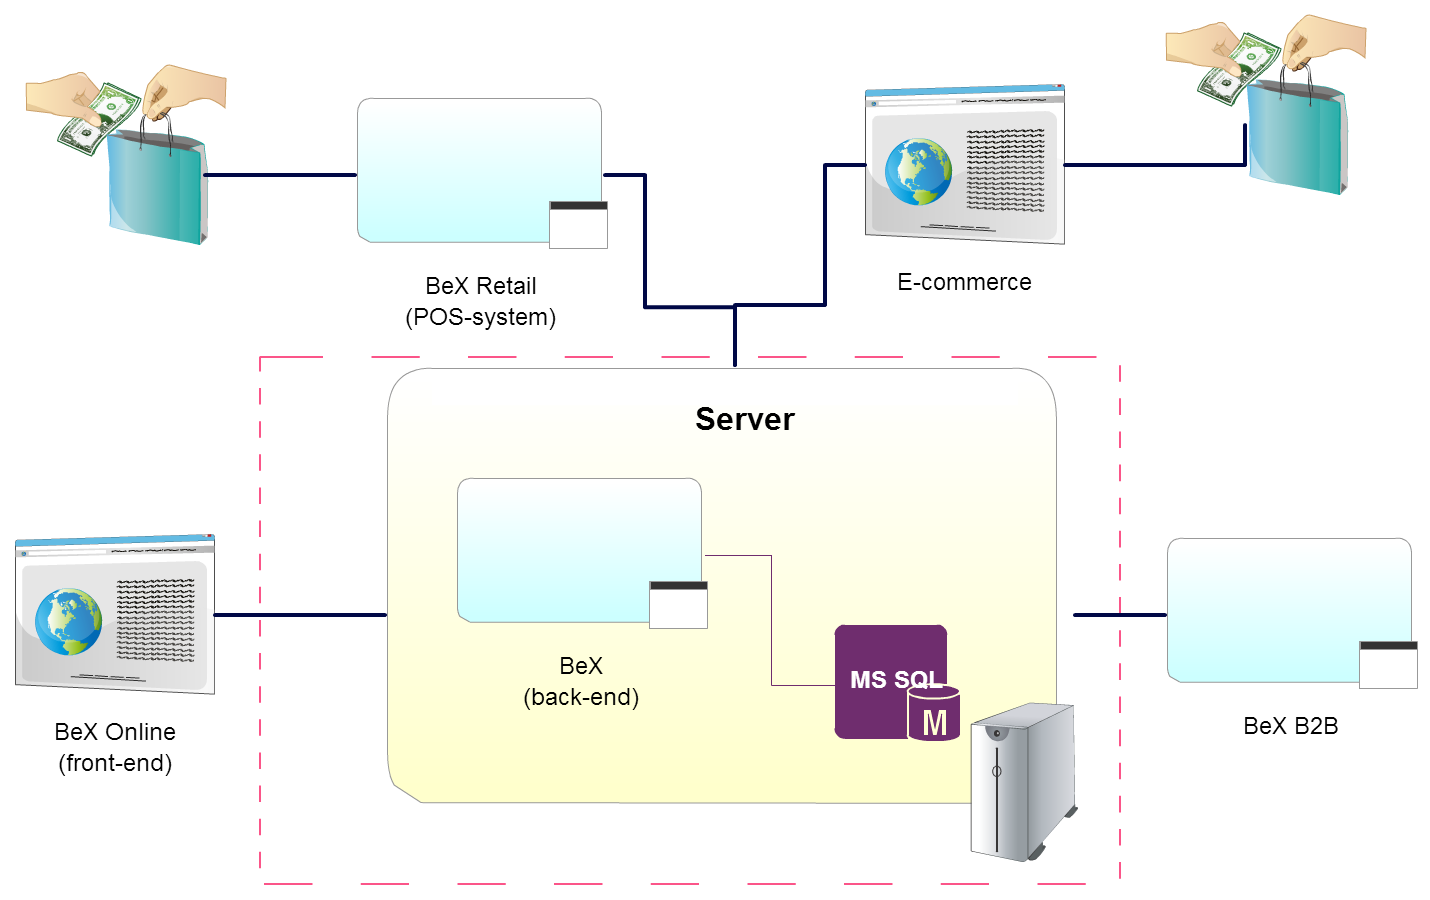
\includegraphics[scale=0.3]{Pictures/Systemdesc.png}
  \end{center}
  \caption{Context diagram of Perfect IT's system}
  \label{context}
  \vspace{-15pt}
\end{figure}
\noindent The dashed section in Figure~\ref{context} are the components that are of the most interest for this thesis and will be more thoroughly described than the other system components.

\subsection{Components}


\subsubsection{Server}
Currently all the clients instances of /bex Online are placed on a single server hosted by a third party hosting company. This server also hosts the database system.
The technical specification of the server is:
\begin{table}[H]
\begin{center}
\begin{tabular}{l l}
OS: & Windows Server 2012 Standard 64-bit\\
CPU: & Intel(R) Xeon(R) CPU E5-2440 @ 2.40 GHz 64-bit based\\
RAM: & 64 GB \\
HD: & 500 GB Disk drive
\end{tabular}
\end{center}
\end{table}

\subsubsection{\bex Online}
\bex Online is a web based system and has a front-end built with HTML5, CSS and JavaScript and a back-end written in C\# and .net with Webforms.
Every client have their own instance of the system \todo{deeper description}

\subsubsection{Database}
The database system used is Microsoft SQL Server 2014 Web edition. It has a maximum data capacity of 524 PB, maximum ram usage of 64GB, maximum CPU capacity < 4 socket or 16 cores. All clients are on the same SQL Server 2014-license but have their own unique instance of the database-system with only their data.  Perfect IT has has around 40 clients, all with different database sizes ranging from approximately 5GB of data to approximately 90GB of data in their database. The database is an RDBMS and is run on a Microsoft SQL Server 2014-license using OLTP and the size of all the clients databases together are approximately 350GB.

\paragraph*{Tables}\mbox{}\\\\
For this thesis Perfect It BeX AB has made available a copy of one of their biggest clients database. To ensure the clients privacy, and the privacy of the clients customers, all sensitive data has been removed. \\ 
The default schema is called \textit{dbo} and consists of a total of 254 tables, including some views for big data queries. Many tables are large, considering the amount of rows, where the largest consists of approximately 10.5$\times 10^6$ rows and 80 columns. This table stores the data associated with every business transaction made by the system from the start of using this system. There are also empty tables, \hilight{usage?}, that \ldots. The tables form a complex relation to each other and the references are many (as seen in this \href{https://drive.google.com/file/d/0B1IYTmE2hnD-eGQ0N2tvYXZNNVE/view?usp=sharing}{\textcolor{blue}{link}}\footnote{https://drive.google.com/file/d/0B1IYTmE2hnD-eGQ0N2tvYXZNNVE/view?usp=sharing}). In the visualized database reference schema there are tables not referencing any tables at all, \hilight{why?}.\\\\ There are also tables needed by third party applications and API's that also are stored in the database and can be seen in the bottom part of the visualized database reference schema mentioned above (\hilight{maybe the answer to the no reference question above?}). Some, \hilight{why not all?} of the BI reports have their own tables in the database, \hilight{why?}.

\paragraph*{Stored procedures}\mbox{}\\\\ 
stored procedures are subroutines that are available to applications that access relational database systems. Stored procedures are used as centralized logic and can therefore be used by all applications that share the system. These subroutines can include both SQL statements and host language statements, meaning that it can exist external procedures that has nothing to do with SQL. Often extensive and complex SQL queries, that require a lot of processing and are often being used, are moved to stored procedures for reuse\cite{StoredProcedures}. It's important to know that stored procedures both bring advantages, e.g. stored procedures are cached, and drawbacks, e.g. stored procedure code is not as robust as app code. Subroutines such as stored procedures should therefore only be used when and if the implementer possess a deep knowledge of the system that is to be affected. It's for example bad practice to store all procedures as stored procedures for the benefit of the cache-utilization.\\\\
The database in this thesis had a total of 59 stored procedures treating repetitive procedures by the database mainly for the sales part of the system and the BI-reports (there's also a subroutine for locking crucial information, with respect to concurrent execution). These subroutines do not contain any host language statements and/or external procedures, but only consists of complex SQL statements. They are present in the system, as mentioned above, to make the execution and processing less demanding, as they are often used in \bex Online.

 
\section{Theory}
In order to understand why a database might not perform optimally, the following theory was used.

\subsection{Index Fragmentation}
Index fragmentation is one of the most common problems in a relational database. Two kinds of fragmentation can occur, internal index fragmentation and external index fragmentation. The easiest way to explain index fragmentation is by imagining the SQL database as a phone book. At the very end of the book you have a few pages containing a table with indexes of all the entries sorted by last name. This is fine in a static environment such as a phone book but what happens in a dynamic environment?
Since people can be added to the phone book there must be space available after each column in the index, as well as in the pages in the phone book. This is called the \emph{fill factor}. A page can still run out of space and when this happens SQL Server has to add a new page, but it it can't add it at the correct place because the book is already bound. So, it adds blank pages at the very end. This causes two problems, pages with a lot of unused space and pages that are out of order. The first problem is what is referred to as \emph{Internal Fragmentation} and the second is \emph{External Fragmentation}. Internal fragmentation will of course also occur when deleting entries since that leaves "blank space" on the page.\cite{Ozar12}

\subsubsection{Why is this bad for performance?}
At first, internal fragmentation might seem like a good thing. If the phone book has a lot of blank space on every page to start with, adding entries would be super easy and there would be no need for adding more pages later, causing external fragmentation. This is true, but when the number of extra pages needed in the phone book to allow for a lot of blank space is considered, the inefficiency of it becomes apparent. Going through a 100\% filled 1000 page phone book is much faster than a 90\% full 1100 page phone book. So in this example, every time SQL Server needs to scan the index, it would take 10\% longer. Another problem is that the lowest unit for caching in SQL Server is not a record, but a single page, which means that all the empty space must be cached as well. \\

External fragmentation often makes reading the database non-sequential, i.e it cannot be read in order but must be read in random order. This is especially bad in classic magnetic hard drives where the reader head must move around to multiple locations on the drive. Some magnetic hard drives only get 1\% of their sequential reading speed when performing random reads.\cite{Toshiba12}

\subsubsection{Measuring fragmentation} \label{measurefrag}
In Al-Farooque Shubho's article "Top 10 ways to optimize data access in SQL Server"\cite{Shubho09} he explains how to measure if index fragmentation has occurred. By executing the script in Algorithm \ref{See DB-Fragmentation} in Appendix \ref{appCode}, index fragmentation is analyzed on every table in the database and presented in a table with an internal and external fragmentation value. \\

According to Shubho, only tables with an internal fragmentation value of less than 75 and/or an external fragmentation value of more than 10 should be considered as fragmented, which this code takes into account.

\subsubsection{Reorganize vs. Rebuild}\mbox{}\\
Both rebuilding and reorganizing are built-in operations in SQL-Server 2014. These are two different operations that both reduce the fragmentation of the indexes. Reorganizing is the more lightweight of the two operations. It fixes the indexes as well as physical reordering of pages and applies any previously set fill factors. Rebuilding builds up a completely new structure for the index. It also allows for a new fill factor.\\
The advantage with reorganizing over rebuilding is that it can be aborted midway, while a rebuild must roll-back after an abort. Usually, in most SQL-systems, a rebuild can't be done while the SQL-server is online. This can be done in MS SQL Server Enterprise edition\cite{Little13}.

\subsubsection{Is it always a good idea to fix fragmentation?}
According to Brent Ozar\cite{Ozar12} fixing fragmentation can cause more damage than keeping fragmented indexes. Often administrators try to fix fragmentation by using a low fill factor, say 50\%. This would mean that half of every page would be blank, which would make writing really fast. Reading however, would be twice as slow. Another common mistake is to rebuild every single index in the database, even though some tables might not had a single write since the last time. This is a problem because defragmenting indexes causes SQL Server to write to the transaction log. The bigger a log is, the longer log backups and restores take.\\\\
Another important factor is that external fragmentation mostly causes problems when the database is stored in disc, since classical hard drives are slow at random reading. If the database is instead stored in memory, which is almost as fast at random reading as sequential reading, external fragmentation won't be as big a issue.

\subsection{Query optimization}\label{sec:qopt}
When talking about query optimization one imagines that the logic in the SQL statements are altered and optimized. Even if this is true, by tuning the actual SQL statements an optimization can be accomplished, it's done with respect to the execution plan. Query optimization can also been seen as mapping of the logical query operations to physical operations that the execution engine can execute.It does this by implementing a number of algorithms, which the query optimizer must choose from when formulating an execution plan. In summary a query optimization is actually a strategic manner to optimize the execution functionality of the execution engine\cite{Nevarez}. \\\\ 
The purpose of the query optimization is to provide a good enough and hopefully optimal execution plan. In order to do so a query must go through a query-processing process as can be viewed in Figure~\ref{fig:qpp}. But before optimizing a query, the SQL Server first checks if there is a execution plan in the cache for the SQL batch. Since the Query optimization is a relative expensive operation, an available execution plan in the cache entails that the optimization process can be skipped as well as the associated cost such as CPU resources and optimization time.\\ The query-processing starts with a simplification of tree representation that is sent from the Algebrizer, which checks the syntax and appropriate bindings of the SQL statement(s). There are 4 stages in the query-processing that return an execution plan and if the simplification of the logic tree representation qualifies as a trivial plan a trivial execution plan is returned and the optimization process ends immediately. Otherwise a full optimization process will be run in up to three stages and an execution plan may be created at the end of any of these stages. All the alternatives the full optimization returns are stored and evaluated by the SQL Server based on the cost. The whole optimization is a cost/benefit trade-off regarding the query optimization time. The number of varying plans can easily rise, an effect known as the combinatorial explosion\cite{combo}, and the optimization will therefore not be feasible as it takes too long. Therefore during this full optimization process the query optimizer uses statistics, transformation rules, heuristics and cost estimations to limit and assure the quality of the executions plans that are returned.\\\\ 
As the query optimizer limits the available alternatives two problems arise. The entire search space is not evaluated and the chosen execution plan is therefore impossible to 
\begin{figure}[H] 
\begin{center}
    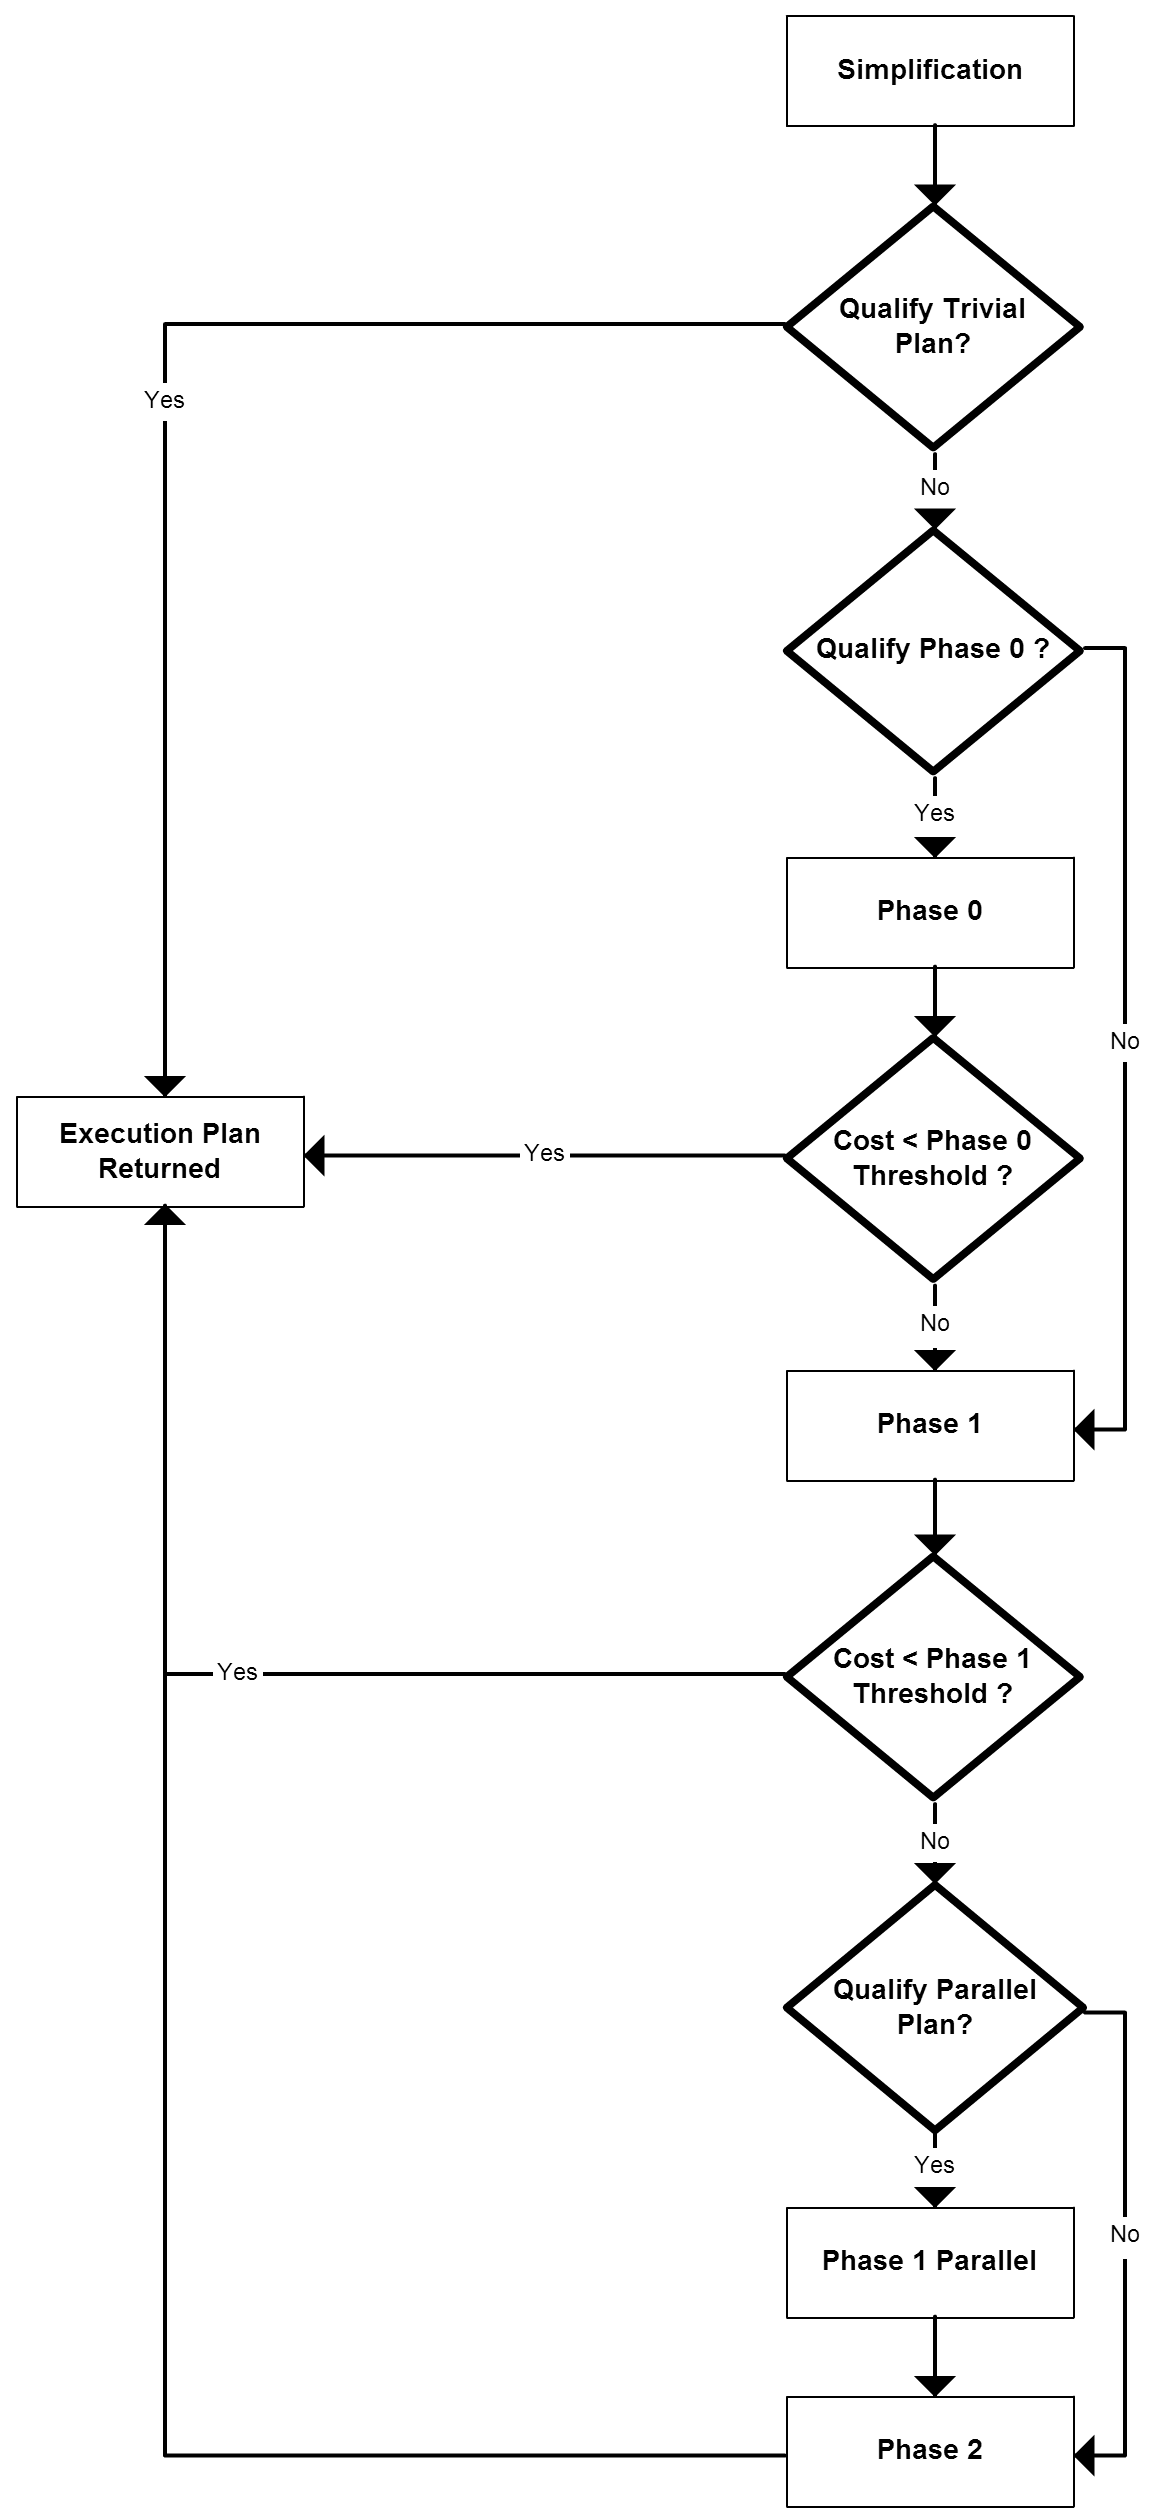
\includegraphics[scale=0.3]{Pictures/Optimization-process.png}
  \end{center}
  \vspace{-20pt}
  \caption{The query-processing process}
  \label{fig:qpp}
  \vspace{-10pt}
\end{figure} 
\noindent prove that it's the most optimal one. So the query optimizers utmost important functionality lies in considering the plans that are of low cost. Which brings us to another major technical challenge, accurate estimations. The quality of the plan that is chosen is only as good as the accuracy of the estimation. According to Nevarez\cite{Nevarez} the estimations are inherently inexact and do not consider the environments hardware conditions. As an example the cost model assumes that every query's data is read from disk and not from memory (cold cache). In addition some operations are not covered by the mathematical model, leading to that the query optimizer has to resort to guessing logic and/or heuristics to deal with such situations. 

\subsubsection{Query tuning}
In order to optimize the process explained above there are numerous areas that can be altered. One can dive in to the actual SQL statements and try to break down complex queries, optimize join ordering etc. Besides altering the SQL statements the workload sent to the query optimizer can be optimized in several ways. Chaudhuri et al. state that compressing the size of a workload, which is a set of SQL statements, improves a systems scalability and illustrates its effectiveness in index selection and approximate query processing\cite{compressing}. Furthermore, major database vendors have focused on releasing automated physical database design tools that reduce the total cost of a workload. An essential assumption of these tools is that the workload consists of a set of SQL statements with no internal ordering. Agrawal et al. state that the workload in itself isn't the most promising aspect of workload optimization, but that the workload can be treated as a sequence which broadens the usage of the above mentioned tools\cite{automatic}.

\paragraph*{Join ordering}\mbox{}\\\\
The order of joins is a key factor in controlling the amount of data flowing between operators in an execution plan. The query optimizer needs to pay close attention to this complex problem and has been the subject of extensive research since the 1970s\cite{join}. The task of the query optimizer is to find the optimal sequence of joins between tables in queries, and the way the joins are ordered can greatly impact the cost and performance of a query. Even though the result of query is the same, disregarding the join order, the cost can vary greatly. Joins have the properties of being both commutative and associative, because of this properties even simple queries can have many different possible join orders and increase exponentially with the number of tables that are involved. As mentioned earlier in section \ref{sec:qopt} the queries are represented as trees in the query processor. The shape of the tree is of utter importance for the query optimizer and is constructed by the nature of the join ordering. In table \ref{table:join} the number of possibilities depending on two sorts of tree shapes (seen in Figure \ref{fig:trees}) are listed, seemingly the number of possibilities increases dramatically. It's obviously impossible for the query optimizer to considerate all this possibilities, it would take too long.  

\begin{figure}[H] 
\begin{center}
    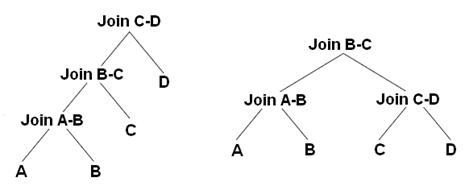
\includegraphics[scale=0.7]{Pictures/trees.jpg}
  \end{center}
  \caption{Left-deep and bushy trees}
  \label{fig:trees}
\end{figure} 
\begin{table}[H]
\centering 
\begin{tabular}{ l l l }
  Tables & Left-Deep Trees (n!) & Bushy Trees (2n-2)!/(n-1)! \\\hline
  2 & 2 & 2 \\\hline
  3 & 6 & 12 \\\hline
  4 & 24 & 120 \\\hline
  5 & 120 & 1 680 \\\hline
  6 & 720 & 30 240 \\\hline
  7 & 5 040 & 665 280 \\\hline
  8 & 40 320 & 17 297 280 \\\hline
  9 & 362 880 & 518 918 400 \\\hline
  10 & 3 628 800 & 17 643 225 600 \\\hline
  11 & 39 916 800 & 670 444 572 800 \\\hline
  12 & 479 001 600 & 28 158 588 057 600 \\
\end{tabular}
\caption {Possible join orders for Left-Deep and Bushy trees}
\label{table:join}
\end{table}

Since the number of the possibilities are that great the query optimizer needs to balance between the optimization time and the quality of it. So the goal of the query optimizer is to find a good enough plan as quick as possible. 

\paragraph*{Query break down}\mbox{}\\\\ \label{querybreakdown}
In some cases the query optimizer may not be able to produce/decide a good plan. This is mostly because of complex queries containing a large number of joins and joins with aggregations. Breaking down these complex queries into two or more and storing the intermediate result in temporary tables is a good plan, since it's fairly rare to request all the data in a single query. 
Howard\cite{break-down} describes several problematic query patterns that the query optimizer has problems creating good plans for. The article is applied to SQL Server versions from 2005 to ''Denali'', but according to Nevarez\cite{Nevarez} it's also applicable to SQL Server 2014.\\ Two important query patterns for this thesis are:
\begin{itemize}
\item OR logic in Where clause
\item Joins on aggregated data sets
\end{itemize}

\subparagraph{\textit{OR} logic in \textit{WHERE} clause}\mbox{}\\\\
When the OR operator is evaluated on one and the same table, e.g. \textit{WHERE a.col1=@val OR a.col2=@val2}, the query optimizer is able to create efficient execution plans by using index seek on two indexes and an index union. However if the \textit{OR} operator is evaluated on different tables, e.g. \textit{WHERE a.col1=@val OR b.col2=@val2}, poor plans may be created. Running the two following queries in Algorithm \ref{firstbreak-down} in Appendix \ref{appCode} will create two efficient plans.\\

If the to tables are joined using the same selective predicates as in Algorithm \ref{firstbreak-down} the SQL Server will return a very expensive plan. This can be fixed by using the \textit{UNION} operator instead of the \textit{OR} operator and allows for seeks on all indexes which results in a more efficient plan, even though the query looks more redundant and complex as seen in Algorithm \ref{second-down} in Appendix \ref{appCode}.


\subparagraph{Joins on aggregated data sets}\mbox{}\\\\
Most large queries join intermediate results from several query blocks involving grouping and aggregation. Earlier aggregation meant grouping of a relation and then apply an aggregate function (e.g. average) on each group. This still applies, but companies and users are not interested in only e.g. the average salary of each department. They want to do further grouping and sorting such as group the above mentioned employees based on their marital status and/or sex\cite{partioned}. Consequently wanting to perform complex processing within each group and grouping among different sets of attributes.\\ A good cardinality estimation can be provided by statistics for operations performed on a table. However, queries using operator such as \textit{GROUP} or \textit{DISTINCT} create result with different number of rows than that are in the stored table. Joining these results on other data sets, statistics on these intermediate results do not exist. If an intermediate result must be materialized before used in a subsequent step statistics are not available. The query optimizer tries to estimate the cardinality based upon the original data set, but since the earlier mentioned operators intermediate result differ from the original data set, the estimation can degrade in accuracy.\\\\ By analyzing the execution plan for theses complex queries, one can partition the query where the estimated number of rows differ a lot from actual number of rows. To ensure statistics, one can store the intermediate results in temporary tables as mentioned in the beginning of this section.     

 
\subsection{In-Memory Database Technology}
Relational database management systems were originally designed in the late 70's\cite{Nevarez}. Because of this, they are designed with the assumption that memory is limited, expensive and that the size of the database is many times larger than the main memory. Today, memory is relatively cheap and it is possible to have hundreds of gigabytes of memory in a single server. This makes it possible to put even large databases, completely in memory. In Vizard's article\cite{Vizard12} it is said that having a database completely in-memory can make it a thousand times faster.

\subsubsection{Hekaton}
Microsoft SQL Server 2014 comes with an In-Memory OLTP database engine called Hekaton. Hekaton, which is only available in the enterprise edition, improves performance in three major architecture areas: Optimization for main memory access, compiling procedures to native code, and latches and lock elimination. The core architecture of Hekaton is a Bw-tree design\cite{Levandoski14}. A Bw-tree is a new design of the classical B-tree which supports high performance in both access to individual keys and key-sequential access to subranges of keys. The Bw-tree is designed for the new hardware environment in two main ways. 
\begin{enumerate}
\item The Bw-tree is latch-free, which is critical for performance when using multi-core systems where latches otherwise are common.
\item Updating cache memory in place in multi-core systems usually results in costly cache invalidations, limiting performance. By performing "delta" updates, the Bw-tree avoids in-place updates which reduces invalidations and preserves previously cached page data.
\end{enumerate} 
The Hekaton engine is not a separate database system, it is fully integrated into SQL Server. A user can declare a table in a current database to be memory-optimized, and the Hekaton engine will store it in main memory and manage it. A Hekaton table can use two different kinds of indexes. Hash indexes and Range indexes.  Even though Hekaton uses very different internal concepts and implementations it still ensures that all transactions have ACID-properties. \\
A big drawback of using Hekaton tables is that the table architecture cannot be altered without recreating the table. This means that in order to change the columns in a table or it's indexing settings, the table must be dropped and then rebuilt from scratch.

\paragraph*{Buckets}\mbox{}\\\\
In Hekaton, Buckets is something you have to reserve for the hash index when creating a memory optimized table. This parameter doesn't exist in when discussing ordinary indexes or other special indexes. Microsoft recommends that one select a bucket count of double the amount of distinct values in the table. The number of buckets also have to be a power of two and the parameter is static once set. This means that the table has to be dropped and rebuild if the bucket count is bad. \\\\
The hash tables in Hekaton are implemented as regular hash tables with keys mapped via a hash function to values. The values are stored in an array of buckets\cite{Barbarin14}. 

\begin{figure}[H]
\begin{center}
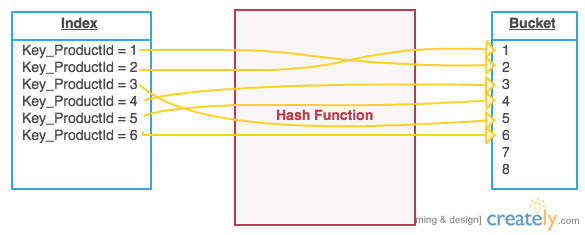
\includegraphics[scale=0.5]{Pictures/buckets.png}
\caption{Illustrating the concept of buckets}
\end{center}
\end{figure}

The hash indexes are in no particular order which makes it ineffective for range operations but fast for lookup operations. The hash function should be efficient enough to spread the keys into the buckets uniformly to avoid multiple values in the same bucket. Multiple values in the same bucket also occurs when there aren't enough buckets. This causes a bucket to have a row chain. This causes the lookup operation to be slower because it has to scan the row chain for the bucket to find the value. The number of keys per bucket is the \emph{load factor} of in-memory tables. This is calculated as the total number of entities divided by the number of buckets. The higher load factor, the slower a table will perform. This means that a fixed bucket count in a table will perform worse over time if the bucket count is too small. However, a too large bucket count will use excess memory and cause range lookups to perform slowly. 

\begin{figure}[H]
\begin{center}
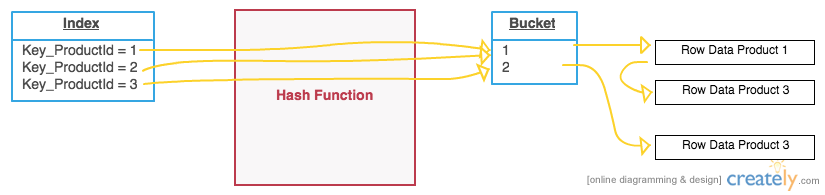
\includegraphics[scale=0.5]{Pictures/buckets2.png}
\caption{Illustrating the concept of a row chain}
\end{center}
\end{figure}

The reason why the bucket count has to be set as a power of two number is to make the hash function faster. The position for a value in a table is calculated as \emph{Hash value \% array size}. The problem with this calculation is that modulo is slow compared to the bit wise AND-operation. By setting the array size, which is the bucket count, to a number that is a power of two, one can use the AND-operation instead and save time.

\paragraph*{Stored procedures in Hekaton}\mbox{}\\\\ 
Hekaton uses the SQL Query Optimizer to produce an efficient query plan. This plane is then compiled into native C code and loaded as DLLs into the SQL Server process. This compilation happens on SQL Server start.
When a procedure is saved as a natively  compiled stored procedure it locks all the tables that it uses. This is because such procedures must be schema bound, i.e all tables referenced by a procedure can't be dropped. If this is considered together with the the limitation mentioned above regarding changing of a table architecture, the following process would be required in order to change e.g. a Hekaton table's columns\cite{Nevarez}.
\begin{enumerate}
\item Drop the procedures referencing the table.
\item Store the data in the Hekaton in a temporary table.
\item Drop the Hekaton table.
\item Rebuild the Hekaton table with the new columns.
\item Reload the data from the temporary table into the new Hekaton table. 
\item Recreate the stored procedures.
\end{enumerate}

A complex procedure like this is preferably avoided. The cost of having to rebuild the in-memory tables from scratch could be high so it is important to plan and choose parameters wisely.


\section{Analysis}
The analysis of the system required several tools and environments for both live and local research, where the local environment setup is further explained in Appendix \ref{Aenviron}. To identify report-relevant parts of the system the tool Microsoft SQL Server Management Studio (SSMS) was mostly used. To identify and study the bottle-necks and problems, in the above mentioned system parts, several other tools such as DBVisualizer, SQL Sentry Plan Explorer etc. were used along side SMSS to extract query duration, query execution plans and much more.\\\\
Much of the analysis revolved around the stored procedures, since it was there the potential of optimization was greatest, but other optimization areas were also studied such as index fragmentation of the relevant tables.      

\subsection{Index fragmentation}
By using the script from the theory the following index fragmentation values were produced. The table names and index names has been changed due to confidentiality.

\begin{table}[H]
\begin{center}
\begin{tabular}{|l|l|l|l|}
\hline
Table name & Index name & External fragmentation & Internal fragmentation \\ \hline 
1  & a & 100         & 74,05485545 \\ \hline
2  & b & 100         & 72,6278725  \\ \hline
3  & c & 100         & 58,68544601 \\ \hline
4  & d & 100         & 70,17500618 \\ \hline
5  & e & 100         & 67,92068199 \\ \hline
6  & f & 100         & 58,46971831 \\ \hline
7  & g & 100         & 50,03706449 \\ \hline
8  & h & 99,48535234 & 57,89085743 \\ \hline
9  & i & 96,11111111 & 73,69038794 \\ \hline
10 & j & 94,44444444 & 70,63737336 \\ \hline
11 & k & 90,59325223 & 52,81183593 \\ \hline
12 & l & 89,13043478 & 65,47550037 \\ \hline
13 & m & 86,99186992 & 65,83502595 \\ \hline
14 & n & 85,71428571 & 47,9579318  \\ \hline
15 & o & 78,98550725 & 57,05273042 \\ \hline
16 & p & 77,77777778 & 56,54531752 \\ \hline
17 & q & 75          & 48,44946874 \\ \hline
18 & r & 73,35790885 & 62,85373116 \\ \hline
19 & j & 71,30559541 & 64,10468248 \\ \hline
20 & s & 69,67213115 & 69,75221151 \\ \hline
21 & m & 68,46173667 & 65,69195701 \\ \hline
22 & t & 67,79506955 & 65,90287868 \\ \hline
23 & u & 66,66666667 & 49,09809736 \\ \hline
24 & v & 50          & 74,49962936 \\ \hline
25 & w & 50          & 53,43464295 \\ \hline
26 & x & 50          & 54,92957746 \\ \hline
27 & y & 50          & 41,83552014 \\ \hline
28 & z & 36,59652333 & 72,06630838 \\ \hline
29 & å & 33,5729147  & 73,20072894 \\ \hline
\end{tabular}
\caption{Results from index fragmentation search}
\end{center}
\end{table}

This shows that some of the indexes used have an external fragmentation well above the value of 10, which is the threshold according to Shubho as mentioned in section \ref{measurefrag}. The internal fragmentation value is also bad at some of the indexes (i.e less than 75).

\subsection{Stored procedures}
As mentioned in the technical description a total of 59 stored procedures are present in the system. A little more than 50\% (30) of these subroutines are directly involved with the BI-reports. In the web interface there are several more reports that can be produced, but the ones not covered by stored procedures are treated in the back-end of the system.  \\\\\todo{Koppla ihop SP till de olika rapporter}
To execute the stored procedures, SQL batches such as Algorithm \ref{spexec} in Appendix \ref{appCode} were produced and executed. The SQL batches simply specifies the essential parameters and the optional ones as wildcards to get a wide range of data as possible.\\\\  
The stored procedures for BI-reports are quite similar considering the block of statements. The majority of the subroutines contain \texttt{SELECT}, \texttt{INSERT}, \texttt{UPDATE} and \texttt{DELETE} SQL block statements with variety in amount and order. The \texttt{SELECT} statements vary greatly in the different stored procedure both in conditions and amount/which tables the data is fetched from. As can been seen in Table \ref{tab:tabfreq} in Appendix \ref{sec:appTabIll} a total of 84 tables are of interest for the BI-report stored procedures and the average amount of tables for a stored procedure is approximately $\approx37$.\\
The data is fetched from the different tables by joining tables on stated conditions and then selected, at most, there is a stored procedure that joins a total of 46 different tables in its execution (see Table \ref{tab:mosttab} in Appendix \ref{sec:appTabIll}). The various stored procedures also have a similarity from which tables the \texttt{JOIN} is done on. Table \ref{tab:tabinall} in Appendix \ref{sec:appTabIll} shows that a total of 26 tables are involved in all of the stored procedures.\\
The fetched data is stored as an intermediate result in a table with a name corresponding to the stored procedure name. This intermediate result table is present by reasons mentioned in \ref{querybreakdown}, with the exception that the table isn't temporary. The table is permanently present in the database due to a previously refactorization of the database by the DBA. The table is therefore meant as an optimization shortcut, where the last queried report result is stored until the same query is executed with different parameters.\\
The intermediate result table is then further altered by updates based on mathematical calculations such as item quantities, contribution margins etc. And in some cases a deletion is performed of rows where the mathematical calculations don't pass the set conditions.   
       
\subsubsection{Execution statistics}
The first step taken to tune the stored procedure was to produce statistics. The goal of our thesis is to speed up the BI-report generation and thereby speeding up the stored procedures. Therefore execution duration was of utter importance and was established with the Transact-SQL \texttt{SET STATISTICS TIME} command, as can be seen in Algorithm \ref{spexec}. This command is used to measure variety of time, some of which may or may not be of much importance considering query tuning. The result varies from query to query and can look something like this: \\\\\texttt{SQL Server parse and compile time:\\
CPU time = 0 ms, elapsed time = 0 ms.\\
SQL Server parse and compile time:\\
CPU time = 0 ms,  elapsed time = 0 ms.\\
SQL Server Execution Times:\\
CPU time = 9002 ms,  elapsed time = 10634 ms.
}\\\\
To explain the above result we first need to clarify the two different measurements CPU-time and elapsed time. The CPU time is a relatively consistent measurement of the amount of CPU resources it takes for a query to run.This is obviously relatively independent of how busy the CPU is on the system the query is run. The elapsed time number is a measurement of how long the whole query took to execute (not including the time for locks or reads). This number is heavily dependent on the server load and can therefore change drastically \cite{statistics}. \\ In the above result example the first measurement block tells us how much time the SQL Server to parse, compile and put the execution plan in cache. The second measurement block tells us the amount of time it took the SQL Server to retrieve the execution plan from the cache. But what is most of interest is the third and frequently last measurement, it's the sum of all earlier measurements and therefore the measurement for the total duration of the query execution. This measurement will help us to determine of the future improvements actually were improvements considering execution speed.\\
The statistics measurements were taken on a system with a quad core processor as seen in Appendix \ref{Aenviron}. Because of this, the CPU-time will in some cases be bigger than the elapsed time since the time stated in the result is then the sum of all busy processors' time. The parse and compile time were all the same for all stored procedures, 0ms, since the environment was established to simulate a live version as close as possible, meaning that almost every table, procedure and execution plan was present in the systems cache. But even though the almost everything was in the system cache, many of the stored procedures execution time were over a comfortable threshold, as can be seen in Table \ref{tab:duration}. 

\begin{table}[H]
\centering
\scalebox{0.9}{
\begin{tabular}{  l | l | l | l  H  H  H  H  H  }
	Stored procedure & \multicolumn{4}{c} {Local} &   Back-End &  & Live &  \\ \hline
	 & CPU (quad core) ms & CPU (single core) ms & elapsed ms & efficiency & CPU & elapsed & CPU & elapsed \\ \hline
	Report 2\_6 & 464372 & 116093 & 427017 & 0.271869738207144 &  &  &  & \  \\ \hline
	Report 2\_5 & 174594 & 43648.5 & 202116 & 0.2159576678738942 &  &  &  & \  \\ \hline
	Report 3\_1 & 138000 & 34500 & 147443 & 0.23398872784737151 &  &  &  & \  \\ \hline
	Report 4\_2 & 35187 & 8796.75 & 33168 & 0.26521798118668594 &  &  &  & \  \\ \hline
	Report 4\_4 & 29187 & 7296.75 & 39300 & 0.18566793893129771 &  &  &  & \  \\ \hline
	Report 1\_1\_2 & 18375 & 4593.75 & 21785 & 0.21086756942850585 &  &  &  & \  \\ \hline
	Report 1\_1\_1 & 9002 & 2250.5 & 10634 & 0.21163249952981003 &  &  &  & \  \\ \hline
	Report 1\_3\_2 & 8343 & 2085.75 & 9522 & 0.21904536862003782 &  &  &  & \  \\ \hline
	Report 4\_3 & 8046 & 2011.5 & 2536 & 0.79317823343848581 &  &  &  & \  \\ \hline
	Report 1\_1\_3 & 7860 & 1965 & 12655 & 0.15527459502173055 &  &  &  & \  \\ \hline
	Report 1\_1\_9 & 7687 & 1921.75 & 8998 & 0.2135752389419871 &  &  &  & \  \\ \hline
	Report 1\_1\_6 & 6813 & 1703.25 & 11381 & 0.14965732360952463 &  &  &  & \  \\ \hline
	Report 1\_1\_7 & 5968 & 1492 & 6429 & 0.23207341732773371 &  &  &  & \  \\ \hline
	Report 1\_1\_4 & 5937 & 1484.25 & 6347 & 0.23385063809673862 &  &  &  & \  \\ \hline
	Report 1\_1\_5 & 5860 & 1465 & 6249 & 0.23443751000160026 &  &  &  & \  \\ \hline
	Report 1\_1\_8 & 5344 & 1336 & 5973 & 0.22367319604888666 &  &  &  & \  \\ \hline
	Report 1\_2\_2 & 4452 & 1113 & 1244 & 0.89469453376205788 &  &  &  & \  \\ \hline
	Report 2\_1\_2 & 3125 & 781.25 & 3433 & 0.22757063792601223 &  &  &  & \  \\ \hline
	Report 1\_5\_7 & 3094 & 773.5 & 5483 & 0.14107240561736276 &  &  &  & \  \\ \hline
	Report 2\_1\_1 & 2360 & 590 & 2650 & 0.22264150943396227 &  &  &  & \  \\ \hline
	Report 4\_5 & 1217 & 304.25 & 3960 & 7.6830808080808083E-2 &  &  &  & \  \\ \hline
	
	\vdots & \vdots & \vdots & \vdots &  &  &  & \  
\end{tabular}}
\caption{Stored procedure execution duration on local database instance}
\label{tab:duration}
\end{table}

In the above table the most crucial stored procedures are listed, considering execution duration. As seen in section \ref{sec:BI} some of the critical reports are the ones that are troublesome time-wise.\\\\
The second Transact-SQL command that was used to produce useful statistics was \texttt{SET STATISTICS ION ON}, also seen in Algorithm \ref{spexec}.  The command provides detailed information about the query's impact on the SQL Server. An example of the output is shown below:\\\\
\texttt{Table 'EXT\_HISTORY\_MASTER'. Scan count 79508, logical reads 1632621, physical reads 0, read-ahead reads 0, lob logical reads 0, lob physical reads 0, lob read-ahead reads 0.}\\\\
Considering query tuning some of this information is helpful, and some not \cite{IO}. The Scan count indicates how many times the referenced table was accessed
\begin{table}[H]
\centering
\scalebox{0.8}{
\begin{tabular}{  l | H  l | l | l | l | l  H H H }

	Stored procedure &  & Object name & Scan count & Logical reads & Physical reads & Read-Ahead Reads & Lob Logical Reads & Lob Physical Reads & Lob read-ahead reads  \  \\ \hline
	3\_1 & Table 'EXT\_SALES\_HEADER'. Scan count 0, logical reads 68850420, physical reads 0, read-ahead reads 0, lob logical reads 0, lob physical reads 0, lob read-ahead reads 0. & EXT\_SALES\_HEADER & 0 & 68850420 & 0 & 0 & 0 & 0 & 0 \\ \hline
	2\_6 & Table 'Worktable'. Scan count 1589989, logical reads 49956351, physical reads 0, read-ahead reads 0, lob logical reads 0, lob physical reads 0, lob read-ahead reads 0. & Worktable & 1589989 & 49956351 & 0 & 0 & 0 & 0 & 0 \\ \hline
	2\_6 & Table 'Worktable'. Scan count 1589989, logical reads 47508411, physical reads 0, read-ahead reads 0, lob logical reads 0, lob physical reads 0, lob read-ahead reads 0. & Worktable & 1589989 & 47508411 & 0 & 0 & 0 & 0 & 0 \\ \hline
	2\_5 & Table 'Worktable'. Scan count 1318326, logical reads 46380365, physical reads 0, read-ahead reads 0, lob logical reads 0, lob physical reads 0, lob read-ahead reads 0. & Worktable & 1318326 & 46380365 & 0 & 0 & 0 & 0 & 0 \\ \hline
	2\_6 & Table 'Worktable'. Scan count 370813, logical reads 40890291, physical reads 0, read-ahead reads 0, lob logical reads 0, lob physical reads 0, lob read-ahead reads 0. & Worktable & 370813 & 40890291 & 0 & 0 & 0 & 0 & 0 \\ \hline
	2\_5 & Table 'EXT\_HISTORY\_MASTER'. Scan count 2257991, logical reads 20336741, physical reads 241, read-ahead reads 27358, lob logical reads 0, lob physical reads 0, lob read-ahead reads 0. & EXT\_HISTORY\_MASTER & 2257991 & 20336741 & 241 & 27358 & 0 & 0 & 0 \\ \hline
	4\_2 & Table 'EXT\_HISTORY\_MASTER'. Scan count 9, logical reads 15318541, physical reads 1940, read-ahead reads 167916, lob logical reads 0, lob physical reads 0, lob read-ahead reads 0. & EXT\_HISTORY\_MASTER & 9 & 15318541 & 1940 & 167916 & 0 & 0 & 0 \\ \hline
	3\_1 & Table 'Worktable'. Scan count 1116354, logical reads 13974108, physical reads 0, read-ahead reads 0, lob logical reads 0, lob physical reads 0, lob read-ahead reads 0. & Worktable & 1116354 & 13974108 & 0 & 0 & 0 & 0 & 0 \\ \hline
	2\_6 & Table 'EXT\_HISTORY\_MASTER'. Scan count 370836, logical reads 13801901, physical reads 1184, read-ahead reads 177558, lob logical reads 0, lob physical reads 0, lob read-ahead reads 0. & EXT\_HISTORY\_MASTER & 370836 & 13801901 & 1184 & 177558 & 0 & 0 & 0 \\ \hline
	2\_6 & Table 'EXT\_ITEM\_LEDGER\_ENTRY'. Scan count 1589989, logical reads 11407484, physical reads 0, read-ahead reads 0, lob logical reads 0, lob physical reads 0, lob read-ahead reads 0. & EXT\_ITEM\_LEDGER\_ENTRY & 1589989 & 11407484 & 0 & 0 & 0 & 0 & 0 \\ \hline
	2\_6 & Table 'EXT\_SALES\_HEADER'. Scan count 5307607, logical reads 10645764, physical reads 0, read-ahead reads 0, lob logical reads 0, lob physical reads 0, lob read-ahead reads 0. & EXT\_SALES\_HEADER & 5307607 & 10645764 & 0 & 0 & 0 & 0 & 0 \\ \hline
	3\_1 & Table 'Worktable'. Scan count 2232708, logical reads 10205255, physical reads 0, read-ahead reads 0, lob logical reads 0, lob physical reads 0, lob read-ahead reads 0. & Worktable & 2232708 & 10205255 & 0 & 0 & 0 & 0 & 0 \\ \hline
	2\_5 & Table 'EXT\_SALES\_HEADER'. Scan count 4868901, logical reads 9765541, physical reads 0, read-ahead reads 0, lob logical reads 0, lob physical reads 0, lob read-ahead reads 0. & EXT\_SALES\_HEADER & 4868901 & 9765541 & 0 & 0 & 0 & 0 & 0 \\ \hline
	2\_5 & Table 'EXT\_ITEM\_LEDGER\_ENTRY'. Scan count 1318326, logical reads 9644543, physical reads 0, read-ahead reads 4, lob logical reads 0, lob physical reads 0, lob read-ahead reads 0. & EXT\_ITEM\_LEDGER\_ENTRY & 1318326 & 9644543 & 0 & 4 & 0 & 0 & 0 \\ \hline
	2\_6 & Table 'Worktable'. Scan count 1589989, logical reads 8500919, physical reads 0, read-ahead reads 0, lob logical reads 0, lob physical reads 0, lob read-ahead reads 0. & Worktable & 1589989 & 8500919 & 0 & 0 & 0 & 0 & 0 \\ \hline
	2\_5 & Table 'Worktable'. Scan count 1318326, logical reads 7530165, physical reads 0, read-ahead reads 0, lob logical reads 0, lob physical reads 0, lob read-ahead reads 0. & Worktable & 1318326 & 7530165 & 0 & 0 & 0 & 0 & 0 \\ \hline
	3\_1 & Table 'EXT\_PURCHASE\_HEADER'. Scan count 0, logical reads 5453698, physical reads 0, read-ahead reads 0, lob logical reads 0, lob physical reads 0, lob read-ahead reads 0. & EXT\_PURCHASE\_HEADER & 0 & 5453698 & 0 & 0 & 0 & 0 & 0 \\ \hline
	2\_6 & Table 'EXT\_REPORT\_RESULT\_2\_6'. Scan count 1, logical reads 4950883, physical reads 0, read-ahead reads 0, lob logical reads 0, lob physical reads 0, lob read-ahead reads 0. & EXT\_REPORT\_RESULT\_2\_6 & 1 & 4950883 & 0 & 0 & 0 & 0 & 0 \\ \hline
	2\_5 & Table 'EXT\_REPORT\_RESULT\_2\_5'. Scan count 1, logical reads 4116135, physical reads 0, read-ahead reads 0, lob logical reads 0, lob physical reads 0, lob read-ahead reads 0. & EXT\_REPORT\_RESULT\_2\_5 & 1 & 4116135 & 0 & 0 & 0 & 0 & 0 \\ \hline
	1\_1\_2 & Table 'EXT\_REPORT\_RESULT\_1\_1\_2'. Scan count 1, logical reads 3811767, physical reads 65, read-ahead reads 63, lob logical reads 0, lob physical reads 0, lob read-ahead reads 0. & EXT\_REPORT\_RESULT\_1\_1\_2 & 1 & 3811767 & 65 & 63 & 0 & 0 & 0 \\ \hline
	1\_5\_7 & Table 'EXT\_SALES\_HEADER'. Scan count 0, logical reads 2117142, physical reads 0, read-ahead reads 0, lob logical reads 0, lob physical reads 0, lob read-ahead reads 0. & EXT\_SALES\_HEADER & 0 & 2117142 & 0 & 0 & 0 & 0 & 0 \\ \hline
	 1\_1\_1 & Table 'EXT\_HISTORY\_MASTER'. Scan count 79508, logical reads 1632621, physical reads 0, read-ahead reads 0, lob logical reads 0, lob physical reads 0, lob read-ahead reads 0. & EXT\_HISTORY\_MASTER & 79508 & 1632621 & 0 & 0 & 0 & 0 & 0 \\ \hline
	1\_1\_2 & Table 'EXT\_HISTORY\_MASTER'. Scan count 79508, logical reads 1632621, physical reads 0, read-ahead reads 0, lob logical reads 0, lob physical reads 0, lob read-ahead reads 0. & EXT\_HISTORY\_MASTER & 79508 & 1632621 & 0 & 0 & 0 & 0 & 0 \\ \hline
	1\_1\_3 & Table 'EXT\_HISTORY\_MASTER'. Scan count 79508, logical reads 1632621, physical reads 0, read-ahead reads 0, lob logical reads 0, lob physical reads 0, lob read-ahead reads 0. & EXT\_HISTORY\_MASTER & 79508 & 1632621 & 0 & 0 & 0 & 0 & 0 \\ \hline
	1\_1\_4 & Table 'EXT\_HISTORY\_MASTER'. Scan count 79508, logical reads 1632621, physical reads 0, read-ahead reads 0, lob logical reads 0, lob physical reads 0, lob read-ahead reads 0. & EXT\_HISTORY\_MASTER & 79508 & 1632621 & 0 & 0 & 0 & 0 & 0 \\ \hline
	1\_1\_5 & Table 'EXT\_HISTORY\_MASTER'. Scan count 79508, logical reads 1632621, physical reads 0, read-ahead reads 0, lob logical reads 0, lob physical reads 0, lob read-ahead reads 0. & EXT\_HISTORY\_MASTER & 79508 & 1632621 & 0 & 0 & 0 & 0 & 0 \\ \hline
	1\_1\_6 & Table 'EXT\_HISTORY\_MASTER'. Scan count 79508, logical reads 1632621, physical reads 0, read-ahead reads 0, lob logical reads 0, lob physical reads 0, lob read-ahead reads 0. & EXT\_HISTORY\_MASTER & 79508 & 1632621 & 0 & 0 & 0 & 0 & 0 \\ \hline
	1\_1\_7 & Table 'EXT\_HISTORY\_MASTER'. Scan count 79508, logical reads 1632621, physical reads 0, read-ahead reads 0, lob logical reads 0, lob physical reads 0, lob read-ahead reads 0. & EXT\_HISTORY\_MASTER & 79508 & 1632621 & 0 & 0 & 0 & 0 & 0 \\ \hline
	1\_1\_8 & Table 'EXT\_HISTORY\_MASTER'. Scan count 79508, logical reads 1632621, physical reads 0, read-ahead reads 0, lob logical reads 0, lob physical reads 0, lob read-ahead reads 0. & EXT\_HISTORY\_MASTER & 79508 & 1632621 & 0 & 0 & 0 & 0 & 0 \\ \hline
	1\_1\_9 & Table 'EXT\_HISTORY\_MASTER'. Scan count 79508, logical reads 1632621, physical reads 0, read-ahead reads 0, lob logical reads 0, lob physical reads 0, lob read-ahead reads 0. & EXT\_HISTORY\_MASTER & 79508 & 1632621 & 0 & 0 & 0 & 0 & 0 \\ \hline
	1\_3\_2 & Table 'EXT\_HISTORY\_MASTER'. Scan count 79508, logical reads 1632621, physical reads 0, read-ahead reads 0, lob logical reads 0, lob physical reads 0, lob read-ahead reads 0. & EXT\_HISTORY\_MASTER & 79508 & 1632621 & 0 & 0 & 0 & 0 & 0 \\ \hline
	1\_3\_2 & Table 'EXT\_HISTORY\_MASTER'. Scan count 79508, logical reads 1632621, physical reads 0, read-ahead reads 0, lob logical reads 0, lob physical reads 0, lob read-ahead reads 0. & EXT\_HISTORY\_MASTER & 79508 & 1632621 & 0 & 0 & 0 & 0 & 0 \\ \hline
	1\_2\_2 & Table 'EXT\_HISTORY\_MASTER'. Scan count 9, logical reads 1445404, physical reads 0, read-ahead reads 0, lob logical reads 0, lob physical reads 0, lob read-ahead reads 0. & EXT\_HISTORY\_MASTER & 9 & 1445404 & 0 & 0 & 0 & 0 & 0 \\ \hline
	2\_5 & Table 'EXT\_ITEM\_LEDGER\_ENTRY'. Scan count 234290, logical reads 1242358, physical reads 0, read-ahead reads 437, lob logical reads 0, lob physical reads 0, lob read-ahead reads 0. & EXT\_ITEM\_LEDGER\_ENTRY & 234290 & 1242358 & 0 & 437 & 0 & 0 & 0 \\ \hline
	2\_6 & Table 'EXT\_REPORT\_RESULT\_2\_6'. Scan count 0, logical reads 1235223, physical reads 0, read-ahead reads 0, lob logical reads 0, lob physical reads 0, lob read-ahead reads 0. & EXT\_REPORT\_RESULT\_2\_6 & 0 & 1235223 & 0 & 0 & 0 & 0 & 0 \\ \hline
	\vdots & \vdots & \vdots & \vdots & \vdots  & \vdots & \vdots & \vdots\ & \vdots & \vdots 
\end{tabular}}
\caption{The top part, sorted by logical reads, of stored procedure execution IO statistics}
\label{tab:IO}
\end{table}
 

\subsubsection{Execution plans}



\chapter{Proposed Solution}\label{sec:proposedsoluton}

\section{Solution Introduction}

\section{Integration}

\chapter{Software Development \& Testing}

\chapter{Discussion}

\chapter{Conclusions}
\addcontentsline{toc}{chapter}{Bibliography}
\bibliographystyle{ieeetr}

\bibliography{MyMSc}

\begin{appendices}

\chapter{Code} \label{appCode}
\begin{lstlisting}[caption={Algorithm to find fragmented tables and the fragmentation values},label=See DB-Fragmentation]
SELECT object_name(dt.object_id) Tablename,si.name
IndexName,dt.avg_fragmentation_in_percent AS
ExternalFragmentation,dt.avg_page_space_used_in_percent AS
InternalFragmentation
FROM
(
    SELECT object_id,index_id,avg_fragmentation_in_percent,avg_page_space_used_in_percent
    FROM sys.dm_db_index_physical_stats (db_id('AdventureWorks'),null,null,null,'DETAILED'
)
WHERE index_id <> 0) AS dt INNER JOIN sys.indexes si ON si.object_id=dt.object_id
AND si.index_id=dt.index_id AND dt.avg_fragmentation_in_percent>10
AND dt.avg_page_space_used_in_percent<75 ORDER BY avg_fragmentation_in_percent DESC
\end{lstlisting}


\begin{lstlisting}[caption={Example of broken-down query, instead of OR operator in WHERE clause on two different tables},label=firstbreak-down]
SELECT SalesOrderID FROM Sales.SalesOrderDetail
WHERE ProductID=897
SELECT SalesOrderID FROM Sales.SalesOrderHeader
WHERE CustomerID=11020
\end{lstlisting}
\newpage

\begin{lstlisting}[caption={UNION instead of OR},label=second-down]
SELECT SalesOrderID FROM Sales.SalesOrderHeader soh
	JOIN Sales.SalesOrderDetail sod
	ON soh.SalesOrderID=sod.SalesOrderID
WHERE sod.ProductID=897
UNION
SELECT SalesOrderID FROM Sales.SalesOrderHeader soh
	JOIN Sales.SalesOrderDetail sod
	ON soh.SalesOrderID=sod.SalesOrderID
WHERE soh.CustomerID=11020
\end{lstlisting} 


\begin{lstlisting}[caption={SQL batch to execute stored procedure report\_2\_5},label=spexec]
USE [bex_bob]
GO
set statistics IO on
set statistics time on
DECLARE	@return_value int

EXEC	@return_value = [dbo].[report_2_5]
		@headerId = 75642,
		@Unit = 10,
		@PurchaseDate1 = '',
		@PurchaseDate2 = '',
		@SalesDate1 = N'2014-01-01',
		@SalesDate2 = N'2015-01-01',
		@StockDate = N'2015-01-01',
		@includeInternal = 1,
		@LocationCode = '',
		@SupplierNo = '',
		@ItemGroupCode = '',
		@ItemCategoryCode = '',
		@ProductGroupCode = '',
		@ProgramCode = '',
		@Collection = '',
		@Gender = -1

SELECT	'Return Value' = @return_value

GO
set statistics IO off
set statistics time off
SELECT * FROM EXT_REPORT_RESULT_2_5
\end{lstlisting}
\chapter{Environments}
\section{General environment}

\section{Analysis environment}\label{Aenviron}
\begin{table}[H]
\begin{center}
\begin{tabular}{l l}
OS: & Windows 8.1 64-bit\\
CPU: & ?\\
RAM: & ?\\
HD: & ? \\
Tools/Programs: & SQL Server Management Studio, SQL Sentry Plan Explorer\\
\end{tabular}
\end{center}
\end{table}
\section{Test environment}

\section{Implementation environment}

\chapter{Large Illustrations and Tables}\label{sec:appTabIll}
\begin{table}[H]
\centering
\scalebox{0.8}{
\begin{tabular}{  l | l | l | l | l | l | l | l  H   H   H   H   H   H   H   H   H   H   H   H   H   H   H   H   H   H   H   H   H   H   H  l | l  }
\LARGE{Table}&\multicolumn{29}{c}{\LARGE{Stored procedure for BI-report}}& \\\hline

	 & 1\_1\_1 & 1\_1\_2 & 1\_1\_3 & 1\_1\_4 & 1\_1\_5 & 1\_1\_6 &1\_1\_7 & 1\_1\_8 & 1\_1\_9 & 1\_2\_2 & 1\_3\_2 & 1\_5\_1 & 1\_5\_2 & 1\_5\_7 & 1\_6\_1 & 2\_1\_1 & 2\_1\_2 & 2\_5 & 2\_6 & 3\_1 & 3\_2 & 3\_3 & 3\_4 & 3\_5 & 3\_6 & 3\_7 & 4\_2 & 4\_3 & 4\_4 & 4\_5 & \dots & TOTAL \\ \hline
	EXT\_BO\_USERS & X & X & X & X & X & X & X & X & X & X & X & X & X & X & X & X & X & X & X & X & X & X & X & X & X & X & X & X & X & X & \dots & 30 \\ \hline
	EXT\_COLLECTION & X & X & X & X & X & X & X & X & X & X & X & X & X & X & X & X & X & X & X & X & X & X & X & X & X & X & X & X & X & X & \dots & 30 \\ \hline
	EXT\_COLOUR\_GROUP & X & X & X & X & X & X & X & X & X & X & X & X & X & X & X & X & X & X & X & X & X & X & X & X & X & X & X & X & X & X  & \dots & 30 \\ \hline
	EXT\_COUNTRY & X & X & X & X & X & X & X & X & X & X & X & X & X & X & X & X & X & X & X & X & X & X & X & X & X & X & X & X & X & X  & \dots & 30 \\ \hline
	EXT\_CUSTOMER & X & X & X & X & X & X & X & X & X & X & X & X & X & X & X & X & X & X & X & X & X & X & X & X & X & X & X & X & X & X  & \dots & 30 \\ \hline
	EXT\_CUSTOMER\_GROUP & X & X & X & X & X & X & X & X & X & X & X & X & X & X & X & X & X & X & X & X & X & X & X & X & X & X & X & X & X & X  & \dots & 30 \\ \hline
	EXT\_CUSTOMER\_INVOICE\_DISCOUNT & X & X & X & X & X & X & X & X & X & X & X & X & X & X & X & X & X & X & X & X & X & X & X & X & X & X & X & X & X & X  & \dots & 30 \\ \hline
	EXT\_CUSTOMER\_POSTING\_GROUP & X & X & X & X & X & X & X & X & X & X & X & X & X & X & X & X & X & X & X & X & X & X & X & X & X & X & X & X & X & X  & \dots & 30 \\ \hline
	EXT\_DIMENSION2 & X & X & X & X & X & X & X & X & X & X & X & X & X & X & X & X & X & X & X & X & X & X & X & X & X & X & X & X & X & X  & \dots & 30 \\ \hline
	EXT\_ITEM & X & X & X & X & X & X & X & X & X & X & X & X & X & X & X & X & X & X & X & X & X & X & X & X & X & X & X & X & X & X  & \dots & 30 \\ \hline
	EXT\_ITEM\_CATEGORY & X & X & X & X & X & X & X & X & X & X & X & X & X & X & X & X & X & X & X & X & X & X & X & X & X & X & X & X & X & X  & \dots & 30 \\ \hline
	EXT\_ITEM\_COMPOSITION & X & X & X & X & X & X & X & X & X & X & X & X & X & X & X & X & X & X & X & X & X & X & X & X & X & X & X & X & X & X  & \dots & 30 \\ \hline
	EXT\_ITEM\_FREIGHTCLASS & X & X & X & X & X & X & X & X & X & X & X & X & X & X & X & X & X & X & X & X & X & X & X & X & X & X & X & X & X & X  & \dots & 30 \\ \hline
	EXT\_ITEM\_GENDER & X & X & X & X & X & X & X & X & X & X & X & X & X & X & X & X & X & X & X & X & X & X & X & X & X & X & X & X & X & X  & \dots & 30 \\ \hline
	EXT\_ITEM\_GROUP & X & X & X & X & X & X & X & X & X & X & X & X & X & X & X & X & X & X & X & X & X & X & X & X & X & X & X & X & X & X  & \dots & 30 \\ \hline
	EXT\_ITEM\_IMPORT & X & X & X & X & X & X & X & X & X & X & X & X & X & X & X & X & X & X & X & X & X & X & X & X & X & X & X & X & X & X  & \dots & 30 \\ \hline
	EXT\_ITEM\_VARIANTS & X & X & X & X & X & X & X & X & X & X & X & X & X & X & X & X & X & X & X & X & X & X & X & X & X & X & X & X & X & X  & \dots & 30 \\ \hline
	EXT\_LENGTH\_GROUP & X & X & X & X & X & X & X & X & X & X & X & X & X & X & X & X & X & X & X & X & X & X & X & X & X & X & X & X & X & X  & \dots & 30 \\ \hline
	EXT\_LOCATIONS & X & X & X & X & X & X & X & X & X & X & X & X & X & X & X & X & X & X & X & X & X & X & X & X & X & X & X & X & X & X  & \dots & 30 \\ \hline
	EXT\_PRODUCT\_GROUP & X & X & X & X & X & X & X & X & X & X & X & X & X & X & X & X & X & X & X & X & X & X & X & X & X & X & X & X & X & X  & \dots & 30 \\ \hline
	EXT\_PROGRAM & X & X & X & X & X & X & X & X & X & X & X & X & X & X & X & X & X & X & X & X & X & X & X & X & X & X & X & X & X & X  & \dots & 30 \\ \hline
	EXT\_REPORT\_HEADER & X & X & X & X & X & X & X & X & X & X & X & X & X & X & X & X & X & X & X & X & X & X & X & X & X & X & X & X & X & X  & \dots & 30 \\ \hline
	EXT\_SALESPERSON & X & X & X & X & X & X & X & X & X & X & X & X & X & X & X & X & X & X & X & X & X & X & X & X & X & X & X & X & X & X  & \dots & 30 \\ \hline
	EXT\_SHOP & X & X & X & X & X & X & X & X & X & X & X & X & X & X & X & X & X & X & X & X & X & X & X & X & X & X & X & X & X & X  & \dots & 30 \\ \hline
	EXT\_SIZE\_GROUP & X & X & X & X & X & X & X & X & X & X & X & X & X & X & X & X & X & X & X & X & X & X & X & X & X & X & X & X & X & X  & \dots & 30 \\ \hline
	EXT\_SUPPLIER & X & X & X & X & X & X & X & X & X & X & X & X & X & X & X & X & X & X & X & X & X & X & X & X & X & X & X & X & X & X  & \dots & 30 \\ \hline
\end{tabular}}
\caption{Most common used tables among stored procedures for BI-reports}
\label{tab:tabinall}
\end{table}


\newgeometry{left=0.2cm, right=0.5cm, bottom=3cm}
\begin{table}[H]
\centering
\resizebox{\textwidth}{!}{
\begin{tabular}{  l | c | c | c | c | c | c | c | c | c | c | c | c | c | c | c | c | c | c | c | c | c | c | c | c | c | c | c | c | c | c | c  }
\LARGE{Table}&\multicolumn{29}{c}{\LARGE{Stored procedure for BI-report}}& \\\hline
	 & 1\_1\_1 & 1\_1\_2 & 1\_1\_3 & 1\_1\_4 & 1\_1\_5 & 1\_1\_6 & 1\_1\_7 & 1\_1\_8 & 1\_1\_9 & 1\_2\_2 & 1\_3\_2 & 1\_5\_1 & 1\_5\_2 & 1\_5\_7 & 1\_6\_1 & 2\_1\_1 & 2\_1\_2 & 2\_5 & 2\_6 & 3\_1 & 3\_2 & 3\_3 & 3\_4 & 3\_5 & 3\_6 & 3\_7 & 4\_2 & 4\_3 & 4\_4 & 4\_5 & TOTAL \\ \hline
	EXT\_ACCOUNT & X & X & X & X & X & X & X & X & X & X & X &  &  &  & X & X & X & X & X &  & X & X & X & X & X &  & X & X & X & X & 25 \\ \hline
	EXT\_BO\_USERS & X & X & X & X & X & X & X & X & X & X & X & X & X & X & X & X & X & X & X & X & X & X & X & X & X & X & X & X & X & X & 30 \\ \hline
	EXT\_COLLECTION & X & X & X & X & X & X & X & X & X & X & X & X & X & X & X & X & X & X & X & X & X & X & X & X & X & X & X & X & X & X & 30 \\ \hline
	EXT\_COLOUR\_GROUP & X & X & X & X & X & X & X & X & X & X & X & X & X & X & X & X & X & X & X & X & X & X & X & X & X & X & X & X & X & X & 30 \\ \hline
	EXT\_COMPANY\_INFORMATION &  &  &  &  &  &  &  &  &  &  &  & X & X & X &  &  &  & X & X & X &  &  &  &  &  & X &  &  &  &  & 7 \\ \hline
	EXT\_COUNTRY & X & X & X & X & X & X & X & X & X & X & X & X & X & X & X & X & X & X & X & X & X & X & X & X & X & X & X & X & X & X & 30 \\ \hline
	EXT\_CUSTOMER & X & X & X & X & X & X & X & X & X & X & X & X & X & X & X & X & X & X & X & X & X & X & X & X & X & X & X & X & X & X & 30 \\ \hline
	EXT\_CUSTOMER\_GROUP & X & X & X & X & X & X & X & X & X & X & X & X & X & X & X & X & X & X & X & X & X & X & X & X & X & X & X & X & X & X & 30 \\ \hline
	EXT\_CUSTOMER\_INVOICE\_DISCOUNT & X & X & X & X & X & X & X & X & X & X & X & X & X & X & X & X & X & X & X & X & X & X & X & X & X & X & X & X & X & X & 30 \\ \hline
	EXT\_CUSTOMER\_LEDGER\_ENTRY & X & X & X & X & X & X & X & X & X & X & X &  &  &  & X & X & X & X & X &  & X & X & X & X & X &  & X & X & X & X & 25 \\ \hline
	EXT\_CUSTOMER\_POSTING\_GROUP & X & X & X & X & X & X & X & X & X & X & X & X & X & X & X & X & X & X & X & X & X & X & X & X & X & X & X & X & X & X & 30 \\ \hline
	EXT\_CUSTOMER\_PRICE\_GROUP &  &  &  &  &  &  &  &  &  &  &  &  &  &  &  &  &  &  &  &  & X &  &  &  &  &  &  &  &  &  & 1 \\ \hline
	EXT\_DELIVERYCHANGE\_REASON &  &  &  &  &  &  &  &  &  &  &  & X & X & X &  &  &  & X & X & X &  &  &  &  &  & X &  &  &  &  & 7 \\ \hline
	EXT\_DIMENSIONX & X & X & X & X & X & X & X & X & X & X & X &  &  &  & X & X & X & X & X &  & X & X & X & X & X &  & X & X & X & X & 25 \\ \hline
	EXT\_DIMENSION2 & X & X & X & X & X & X & X & X & X & X & X & X & X & X & X & X & X & X & X & X & X & X & X & X & X & X & X & X & X & X & 30 \\ \hline
	EXT\_DISC\_CODE &  &  &  &  &  &  &  &  &  &  & X &  &  &  &  &  &  &  &  &  &  &  &  &  &  &  &  &  &  &  & 1 \\ \hline
	EXT\_HISTORY\_MASTER & X & X & X & X & X & X & X & X & X & X & X &  &  &  & X & X & X & X & X &  & X & X & X & X & X &  & X & X & X & X & 25 \\ \hline
	EXT\_ITEM & X & X & X & X & X & X & X & X & X & X & X & X & X & X & X & X & X & X & X & X & X & X & X & X & X & X & X & X & X & X & 30 \\ \hline
	EXT\_ITEM\_CATEGORY & X & X & X & X & X & X & X & X & X & X & X & X & X & X & X & X & X & X & X & X & X & X & X & X & X & X & X & X & X & X & 30 \\ \hline
	EXT\_ITEM\_COMPOSITION & X & X & X & X & X & X & X & X & X & X & X & X & X & X & X & X & X & X & X & X & X & X & X & X & X & X & X & X & X & X & 30 \\ \hline
	EXT\_ITEM\_FREIGHTCLASS & X & X & X & X & X & X & X & X & X & X & X & X & X & X & X & X & X & X & X & X & X & X & X & X & X & X & X & X & X & X & 30 \\ \hline
	EXT\_ITEM\_GENDER & X & X & X & X & X & X & X & X & X & X & X & X & X & X & X & X & X & X & X & X & X & X & X & X & X & X & X & X & X & X & 30 \\ \hline
	EXT\_ITEM\_GROUP & X & X & X & X & X & X & X & X & X & X & X & X & X & X & X & X & X & X & X & X & X & X & X & X & X & X & X & X & X & X & 30 \\ \hline
	EXT\_ITEM\_IMPORT & X & X & X & X & X & X & X & X & X & X & X & X & X & X & X & X & X & X & X & X & X & X & X & X & X & X & X & X & X & X & 30 \\ \hline
	EXT\_ITEM\_LEDGER\_ENTRY & X & X & X & X & X & X & X & X & X & X & X &  &  &  & X & X & X & X & X & X & X & X & X & X & X & X & X & X & X & X & 27 \\ \hline
	EXT\_ITEM\_VARIANTS & X & X & X & X & X & X & X & X & X & X & X & X & X & X & X & X & X & X & X & X & X & X & X & X & X & X & X & X & X & X & 30 \\ \hline
	EXT\_LENGTH\_GROUP & X & X & X & X & X & X & X & X & X & X & X & X & X & X & X & X & X & X & X & X & X & X & X & X & X & X & X & X & X & X & 30 \\ \hline
	EXT\_LOCATIONS & X & X & X & X & X & X & X & X & X & X & X & X & X & X & X & X & X & X & X & X & X & X & X & X & X & X & X & X & X & X & 30 \\ \hline
	EXT\_ORDER\_TYPE &  &  &  &  &  &  &  &  &  &  &  & X & X & X &  &  &  & X & X & X &  &  &  &  &  & X &  &  &  &  & 7 \\ \hline
	EXT\_POSTING\_GROUP\_ITEM & X & X & X & X & X & X & X & X & X & X & X &  &  &  & X & X & X & X & X &  & X & X & X & X & X &  & X & X & X & X & 25 \\ \hline
	EXT\_POSTING\_SETUP &  &  &  &  &  &  &  &  &  &  &  &  &  &  &  &  &  &  &  &  & X &  &  &  &  &  &  &  &  &  & 1 \\ \hline
	EXT\_PRODUCT\_GROUP & X & X & X & X & X & X & X & X & X & X & X & X & X & X & X & X & X & X & X & X & X & X & X & X & X & X & X & X & X & X & 30 \\ \hline
	EXT\_PROGRAM & X & X & X & X & X & X & X & X & X & X & X & X & X & X & X & X & X & X & X & X & X & X & X & X & X & X & X & X & X & X & 30 \\ \hline
	EXT\_PURCHASE\_HEADER &  &  &  &  &  &  &  &  &  &  &  & X & X & X &  &  &  & X & X & X &  &  &  &  &  & X &  &  &  &  & 7 \\ \hline
	EXT\_PURCHASE\_LINE &  &  &  &  &  &  &  &  &  &  &  & X & X & X &  &  &  & X & X & X &  &  &  &  &  & X &  &  &  &  & 7 \\ \hline
	EXT\_REATAIL\_CUSTCERTS &  &  &  &  &  &  &  &  &  &  &  & X & X & X &  &  &  & X & X & X &  &  &  &  &  & X &  &  &  &  & 7 \\ \hline
	EXT\_REPORT\_HEADER & X & X & X & X & X & X & X & X & X & X & X & X & X & X & X & X & X & X & X & X & X & X & X & X & X & X & X & X & X & X & 30 \\ \hline
	EXT\_REPORT\_RESULT\_1\_1\_1 & X &  &  &  &  &  &  &  &  &  &  &  &  &  &  &  &  &  &  &  &  &  &  &  &  &  &  &  &  &  & 1 \\ \hline
	EXT\_REPORT\_RESULT\_1\_1\_2 &  & X &  &  &  &  &  &  &  &  &  &  &  &  &  &  &  &  &  &  &  &  &  &  &  &  &  &  &  &  & 1 \\ \hline
	EXT\_REPORT\_RESULT\_1\_1\_3 &  &  & X &  &  &  &  &  &  &  &  &  &  &  &  &  &  &  &  &  &  &  &  &  &  &  &  &  &  &  & 1 \\ \hline
	EXT\_REPORT\_RESULT\_1\_1\_4 &  &  &  & X &  &  &  &  &  &  &  &  &  &  &  &  &  &  &  &  &  &  &  &  &  &  &  &  &  &  & 1 \\ \hline
	EXT\_REPORT\_RESULT\_1\_1\_5 &  &  &  &  & X &  &  &  &  &  &  &  &  &  &  &  &  &  &  &  &  &  &  &  &  &  &  &  &  &  & 1 \\ \hline
	EXT\_REPORT\_RESULT\_1\_1\_6 &  &  &  &  &  & X &  &  &  &  &  &  &  &  &  &  &  &  &  &  &  &  &  &  &  &  &  &  &  &  & 1 \\ \hline
	EXT\_REPORT\_RESULT\_1\_1\_7 &  &  &  &  &  &  & X &  &  &  &  &  &  &  &  &  &  &  &  &  &  &  &  &  &  &  &  &  &  &  & 1 \\ \hline
	EXT\_REPORT\_RESULT\_1\_1\_8 &  &  &  &  &  &  &  & X &  &  &  &  &  &  &  &  &  &  &  &  &  &  &  &  &  &  &  &  &  &  & 1 \\ \hline
	EXT\_REPORT\_RESULT\_1\_1\_9 &  &  &  &  &  &  &  &  & X &  &  &  &  &  &  &  &  &  &  &  &  &  &  &  &  &  &  &  &  &  & 1 \\ \hline
	EXT\_REPORT\_RESULT\_1\_2\_2 &  &  &  &  &  &  &  &  &  & X &  &  &  &  &  &  &  &  &  &  &  &  &  &  &  &  &  &  &  &  & 1 \\ \hline
	EXT\_REPORT\_RESULT\_1\_3\_2 &  &  &  &  &  &  &  &  &  &  & X &  &  &  &  &  &  &  &  &  &  &  &  &  &  &  &  &  &  &  & 1 \\ \hline
	EXT\_REPORT\_RESULT\_1\_5\_1 &  &  &  &  &  &  &  &  &  &  &  & X &  &  &  &  &  &  &  &  &  &  &  &  &  &  &  &  &  &  & 1 \\ \hline
	EXT\_REPORT\_RESULT\_1\_5\_2 &  &  &  &  &  &  &  &  &  &  &  &  & X &  &  &  &  &  &  &  &  &  &  &  &  &  &  &  &  &  & 1 \\ \hline
	EXT\_REPORT\_RESULT\_1\_5\_7 &  &  &  &  &  &  &  &  &  &  &  &  &  & X &  &  &  &  &  &  &  &  &  &  &  &  &  &  &  &  & 1 \\ \hline
	EXT\_REPORT\_RESULT\_1\_6\_1 &  &  &  &  &  &  &  &  &  &  &  &  &  &  & X &  &  &  &  &  &  &  &  &  &  &  &  &  &  &  & 1 \\ \hline
	EXT\_REPORT\_RESULT\_2\_1\_1 &  &  &  &  &  &  &  &  &  &  &  &  &  &  &  & X &  &  &  &  &  &  &  &  &  &  &  &  &  &  & 1 \\ \hline
	EXT\_REPORT\_RESULT\_2\_1\_2 &  &  &  &  &  &  &  &  &  &  &  &  &  &  &  &  & X &  &  &  &  &  &  &  &  &  &  &  &  &  & 1 \\ \hline
	EXT\_REPORT\_RESULT\_2\_5 &  &  &  &  &  &  &  &  &  &  &  &  &  &  &  &  &  & X &  &  &  &  &  &  &  &  &  &  &  &  & 1 \\ \hline
	EXT\_REPORT\_RESULT\_2\_6 &  &  &  &  &  &  &  &  &  &  &  &  &  &  &  &  &  &  & X &  &  &  &  &  &  &  &  &  &  &  & 1 \\ \hline
	EXT\_REPORT\_RESULT\_3\_1 &  &  &  &  &  &  &  &  &  &  &  &  &  &  &  &  &  &  &  & X &  &  &  &  &  &  &  &  &  &  & 1 \\ \hline
	EXT\_REPORT\_RESULT\_3\_2 &  &  &  &  &  &  &  &  &  &  &  &  &  &  &  &  &  &  &  &  & X &  &  &  &  &  &  &  &  &  & 1 \\ \hline
	EXT\_REPORT\_RESULT\_3\_3 &  &  &  &  &  &  &  &  &  &  &  &  &  &  &  &  &  &  &  &  &  & X &  &  &  &  &  &  &  &  & 1 \\ \hline
	EXT\_REPORT\_RESULT\_3\_4 &  &  &  &  &  &  &  &  &  &  &  &  &  &  &  &  &  &  &  &  &  &  & X &  &  &  &  &  &  &  & 1 \\ \hline
	EXT\_REPORT\_RESULT\_3\_5 &  &  &  &  &  &  &  &  &  &  &  &  &  &  &  &  &  &  &  &  &  &  &  & X &  &  &  &  &  &  & 1 \\ \hline
	EXT\_REPORT\_RESULT\_3\_6 &  &  &  &  &  &  &  &  &  &  &  &  &  &  &  &  &  &  &  &  &  &  &  &  & X &  &  &  &  &  & 1 \\ \hline
	EXT\_REPORT\_RESULT\_3\_7 &  &  &  &  &  &  &  &  &  &  &  &  &  &  &  &  &  &  &  &  &  &  &  &  &  & X &  &  &  &  & 1 \\ \hline
	EXT\_REPORT\_RESULT\_3\_7\_SUB1 &  &  &  &  &  &  &  &  &  &  &  &  &  &  &  &  &  &  &  &  &  &  &  &  &  & X &  &  &  &  & 1 \\ \hline
	EXT\_REPORT\_RESULT\_4\_2 &  &  &  &  &  &  &  &  &  &  &  &  &  &  &  &  &  &  &  &  &  &  &  &  &  &  & X &  &  &  & 1 \\ \hline
	EXT\_REPORT\_RESULT\_4\_3 &  &  &  &  &  &  &  &  &  &  &  &  &  &  &  &  &  &  &  &  &  &  &  &  &  &  &  & X &  &  & 1 \\ \hline
	EXT\_REPORT\_RESULT\_4\_4 &  &  &  &  &  &  &  &  &  &  &  &  &  &  &  &  &  &  &  &  &  &  &  &  &  &  &  &  & X &  & 1 \\ \hline
	EXT\_REPORT\_RESULT\_4\_5 &  &  &  &  &  &  &  &  &  &  &  &  &  &  &  &  &  &  &  &  &  &  &  &  &  &  &  &  &  & X & 1 \\ \hline
	EXT\_RETURN\_REASONS & X & X & X & X & X & X & X & X & X & X & X &  &  &  & X & X & X & X & X & X & X & X & X & X & X & X & X & X & X & X & 27 \\ \hline
	EXT\_SALES\_HEADER &  &  &  &  &  &  &  &  &  &  &  & X & X & X &  &  &  & X & X & X &  &  &  &  &  & X &  &  &  &  & 7 \\ \hline
	EXT\_SALES\_LINE &  &  &  &  &  &  &  &  &  &  &  & X & X & X &  &  &  & X & X & X &  &  &  &  &  & X &  &  &  &  & 7 \\ \hline
	EXT\_SALES\_PRICE &  &  &  &  &  &  &  &  &  &  &  &  &  &  &  &  &  &  &  &  & X &  &  &  &  &  &  &  &  &  & 1 \\ \hline
	EXT\_SALESPERSON & X & X & X & X & X & X & X & X & X & X & X & X & X & X & X & X & X & X & X & X & X & X & X & X & X & X & X & X & X & X & 30 \\ \hline
	EXT\_SHIPPING\_AGENT &  &  &  &  &  &  &  &  &  &  &  & X & X & X &  &  &  & X & X & X &  &  &  &  &  & X &  &  &  &  & 7 \\ \hline
	EXT\_SHIPPING\_AGENT\_SERVICE &  &  &  &  &  &  &  &  &  &  &  & X & X & X &  &  &  & X & X & X &  &  &  &  &  & X &  &  &  &  & 7 \\ \hline
	EXT\_SHOP & X & X & X & X & X & X & X & X & X & X & X & X & X & X & X & X & X & X & X & X & X & X & X & X & X & X & X & X & X & X & 30 \\ \hline
	EXT\_SIZE\_GROUP & X & X & X & X & X & X & X & X & X & X & X & X & X & X & X & X & X & X & X & X & X & X & X & X & X & X & X & X & X & X & 30 \\ \hline
	EXT\_SUPPLIER & X & X & X & X & X & X & X & X & X & X & X & X & X & X & X & X & X & X & X & X & X & X & X & X & X & X & X & X & X & X & 30 \\ \hline
	EXT\_SUPPLIER\_GIROPAYMENT & X & X & X & X & X & X & X & X & X & X & X &  &  &  & X & X & X & X & X &  & X & X & X & X & X &  & X & X & X & X & 25 \\ \hline
	EXT\_SUPPLIER\_LEDGER\_ENTRY & X & X & X & X & X & X & X & X & X & X & X &  &  &  & X & X & X & X & X &  & X & X & X & X & X &  & X & X & X & X & 25 \\ \hline
	EXT\_TIMETRACKER &  &  &  &  &  &  &  &  &  &  &  &  &  &  & X &  &  &  &  &  &  &  &  &  &  &  &  &  &  &  & 1 \\ \hline
	EXT\_TIMETRACKER\_WORKCODE &  &  &  &  &  &  &  &  &  &  &  &  &  &  & X &  &  &  &  &  &  &  &  &  &  &  &  &  &  &  & 1 \\ \hline
	TOTAL & 36 & 36 & 36 & 36 & 36 & 36 & 36 & 36 & 36 & 36 & 37 & 37 & 37 & 37 & 38 & 36 & 36 & 46 & 46 & 39 & 39 & 36 & 36 & 36 & 36 & 40 & 36 & 36 & 36 & 36 & \  
\end{tabular}}
\caption{The frequency of table-use in the stored
\label{tab:tabfreq} procedures}
\end{table}
\restoregeometry

\begin{table}[H]
\centering
\scalebox{0.5}{

\begin{tabular}{ l | p{5em} | p{5em}| p{5em}| p{5em}| l  }
\LARGE{Table}&\multicolumn{4}{c}{\LARGE{Stored procedure for BI-report}}& \\\hline
	 & 2\_5 & 2\_6 & 3\_7 & 3\_1 & 3\_2 \\ \hline
	EXT\_BO\_USERS & X & X & X & X & X \\ \hline
	EXT\_COLLECTION & X & X & X & X & X \\ \hline
	EXT\_COLOUR\_GROUP & X & X & X & X & X \\ \hline
	EXT\_COUNTRY & X & X & X & X & X \\ \hline
	EXT\_CUSTOMER & X & X & X & X & X \\ \hline
	EXT\_CUSTOMER\_GROUP & X & X & X & X & X \\ \hline
	EXT\_CUSTOMER\_INVOICE\_DISCOUNT & X & X & X & X & X \\ \hline
	EXT\_CUSTOMER\_POSTING\_GROUP & X & X & X & X & X \\ \hline
	EXT\_DIMENSION2 & X & X & X & X & X \\ \hline
	EXT\_ITEM & X & X & X & X & X \\ \hline
	EXT\_ITEM\_CATEGORY & X & X & X & X & X \\ \hline
	EXT\_ITEM\_COMPOSITION & X & X & X & X & X \\ \hline
	EXT\_ITEM\_FREIGHTCLASS & X & X & X & X & X \\ \hline
	EXT\_ITEM\_GENDER & X & X & X & X & X \\ \hline
	EXT\_ITEM\_GROUP & X & X & X & X & X \\ \hline
	EXT\_ITEM\_IMPORT & X & X & X & X & X \\ \hline
	EXT\_ITEM\_VARIANTS & X & X & X & X & X \\ \hline
	EXT\_LENGTH\_GROUP & X & X & X & X & X \\ \hline
	EXT\_LOCATIONS & X & X & X & X & X \\ \hline
	EXT\_PRODUCT\_GROUP & X & X & X & X & X \\ \hline
	EXT\_PROGRAM & X & X & X & X & X \\ \hline
	EXT\_REPORT\_HEADER & X & X & X & X & X \\ \hline
	EXT\_SALESPERSON & X & X & X & X & X \\ \hline
	EXT\_SHOP & X & X & X & X & X \\ \hline
	EXT\_SIZE\_GROUP & X & X & X & X & X \\ \hline
	EXT\_SUPPLIER & X & X & X & X & X \\ \hline
	EXT\_ITEM\_LEDGER\_ENTRY & X & X & X & X & X \\ \hline
	EXT\_RETURN\_REASONS & X & X & X & X & X \\ \hline
	EXT\_ACCOUNT & X & X &  &  & X \\ \hline
	EXT\_CUSTOMER\_LEDGER\_ENTRY & X & X &  &  & X \\ \hline
	EXT\_DIMENSIONX & X & X &  &  & X \\ \hline
	EXT\_HISTORY\_MASTER & X & X &  &  & X \\ \hline
	EXT\_POSTING\_GROUP\_ITEM & X & X &  &  & X \\ \hline
	EXT\_SUPPLIER\_GIROPAYMENT & X & X &  &  & X \\ \hline
	EXT\_SUPPLIER\_LEDGER\_ENTRY & X & X &  &  & X \\ \hline
	EXT\_COMPANY\_INFORMATION & X & X & X & X &  \\ \hline
	EXT\_DELIVERYCHANGE\_REASON & X & X & X & X &  \\ \hline
	EXT\_ORDER\_TYPE & X & X & X & X &  \\ \hline
	EXT\_PURCHASE\_HEADER & X & X & X & X &  \\ \hline
	EXT\_PURCHASE\_LINE & X & X & X & X &  \\ \hline
	EXT\_REATAIL\_CUSTCERTS & X & X & X & X &  \\ \hline
	EXT\_SALES\_HEADER & X & X & X & X &  \\ \hline
	EXT\_SALES\_LINE & X & X & X & X &  \\ \hline
	EXT\_SHIPPING\_AGENT & X & X & X & X &  \\ \hline
	EXT\_SHIPPING\_AGENT\_SERVICE & X & X & X & X &  \\ \hline
	EXT\_CUSTOMER\_PRICE\_GROUP &  &  &  &  & X \\ \hline
	EXT\_DISC\_CODE &  &  &  &  &  \\ \hline
	EXT\_POSTING\_SETUP &  &  &  &  & X \\ \hline
	EXT\_REPORT\_RESULT\_1\_1\_1 &  &  &  &  &  \\ \hline
	EXT\_REPORT\_RESULT\_1\_1\_2 &  &  &  &  &  \\ \hline
	EXT\_REPORT\_RESULT\_1\_1\_3 &  &  &  &  &  \\ \hline
	EXT\_REPORT\_RESULT\_1\_1\_4 &  &  &  &  &  \\ \hline
	EXT\_REPORT\_RESULT\_1\_1\_5 &  &  &  &  &  \\ \hline
	EXT\_REPORT\_RESULT\_1\_1\_6 &  &  &  &  &  \\ \hline
	EXT\_REPORT\_RESULT\_1\_1\_7 &  &  &  &  &  \\ \hline
	EXT\_REPORT\_RESULT\_1\_1\_8 &  &  &  &  &  \\ \hline
	EXT\_REPORT\_RESULT\_1\_1\_9 &  &  &  &  &  \\ \hline
	EXT\_REPORT\_RESULT\_1\_2\_2 &  &  &  &  &  \\ \hline
	EXT\_REPORT\_RESULT\_1\_3\_2 &  &  &  &  &  \\ \hline
	EXT\_REPORT\_RESULT\_1\_5\_1 &  &  &  &  &  \\ \hline
	EXT\_REPORT\_RESULT\_1\_5\_2 &  &  &  &  &  \\ \hline
	EXT\_REPORT\_RESULT\_1\_5\_7 &  &  &  &  &  \\ \hline
	EXT\_REPORT\_RESULT\_1\_6\_1 &  &  &  &  &  \\ \hline
	EXT\_REPORT\_RESULT\_2\_1\_1 &  &  &  &  &  \\ \hline
	EXT\_REPORT\_RESULT\_2\_1\_2 &  &  &  &  &  \\ \hline
	EXT\_REPORT\_RESULT\_2\_5 & X &  &  &  &  \\ \hline
	EXT\_REPORT\_RESULT\_2\_6 &  & X &  &  &  \\ \hline
	EXT\_REPORT\_RESULT\_3\_1 &  &  &  & X &  \\ \hline
	EXT\_REPORT\_RESULT\_3\_2 &  &  &  &  & X \\ \hline
	EXT\_REPORT\_RESULT\_3\_3 &  &  &  &  &  \\ \hline
	EXT\_REPORT\_RESULT\_3\_4 &  &  &  &  &  \\ \hline
	EXT\_REPORT\_RESULT\_3\_5 &  &  &  &  &  \\ \hline
	EXT\_REPORT\_RESULT\_3\_6 &  &  &  &  &  \\ \hline
	EXT\_REPORT\_RESULT\_3\_7 &  &  & X &  &  \\ \hline
	EXT\_REPORT\_RESULT\_3\_7\_SUB1 &  &  & X &  &  \\ \hline
	EXT\_REPORT\_RESULT\_4\_2 &  &  &  &  &  \\ \hline
	EXT\_REPORT\_RESULT\_4\_3 &  &  &  &  &  \\ \hline
	EXT\_REPORT\_RESULT\_4\_4 &  &  &  &  &  \\ \hline
	EXT\_REPORT\_RESULT\_4\_5 &  &  &  &  &  \\ \hline
	EXT\_SALES\_PRICE &  &  &  &  & X \\ \hline
	EXT\_TIMETRACKER &  &  &  &  &  \\ \hline
	EXT\_TIMETRACKER\_WORKCODE &  &  &  &  &  \\ \hline
	TOTAL & 46 & 46 & 40 & 39 & 39 \\ \hline

\end{tabular}}
\caption{Most tables used among stored procedures for BI-reports}
\label{tab:mosttab}
\end{table}


\begin{figure}[H]
\centering
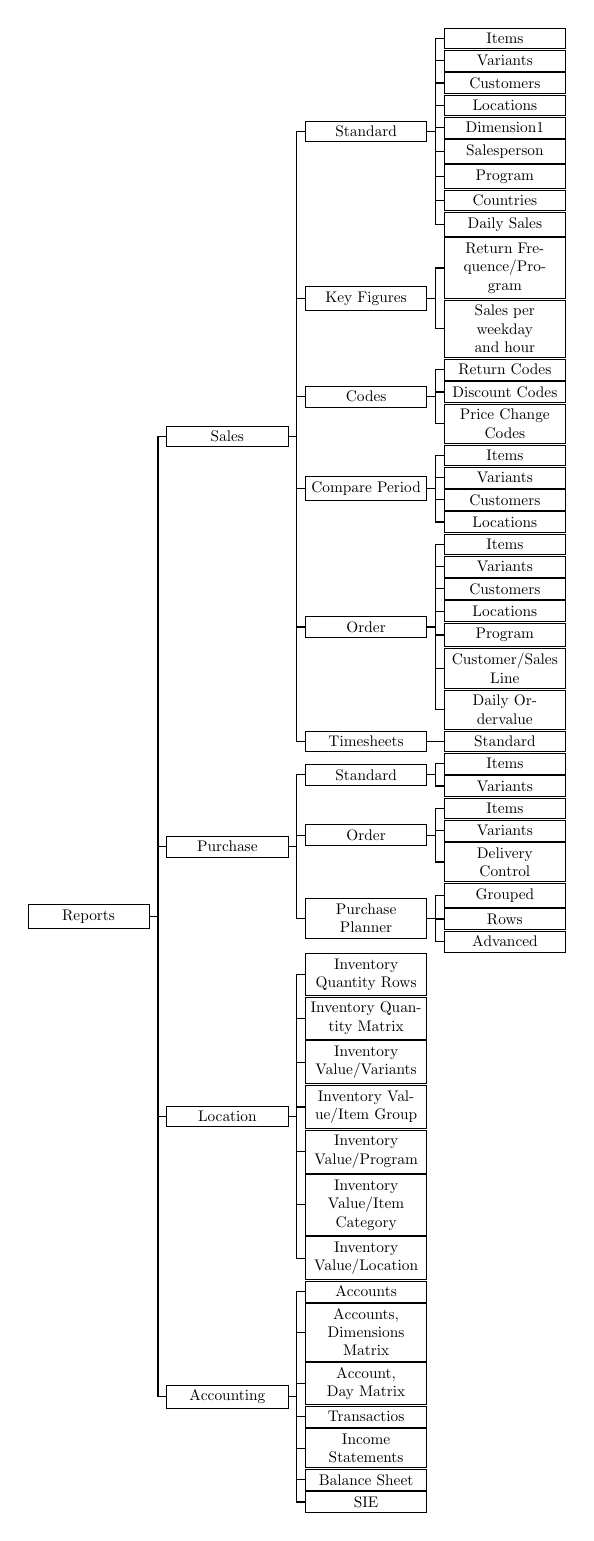
\begin{tikzpicture}[level distance=1.25in,sibling distance=.6pt,scale=.555]
\tikzset{edge from parent/.style= 
            {thick, draw,
                edge from parent fork right},every tree node/.style={draw,minimum width=1in,text width=1in, align=center},grow'=right}
\Tree 
    [. Reports 
        [.{Sales}
            [.{Standard} 
				[.{Items} ]
            	[.{Variants} ]
            	[.{Customers} ]
            	[.{Locations} ]
            	[.{Dimension1} ]
            	[.{Salesperson} ]
            	[.{Program} ]
            	[.{Countries} ]
            	[.{Daily Sales} ]                        
            ]
            [.{Key Figures} 
				[.{Return Frequence/Program} ]
            	[.{Sales per weekday and hour } ]            
            ]
            [.{Codes} 
            	[.{Return Codes} ]
            	[.{Discount Codes} ]
            	[.{Price Change Codes} ]                   
            ]
            [.{Compare Period} 
				[.{Items} ]
            	[.{Variants} ]
            	[.{Customers} ]
            	[.{Locations} ]             
            ]
            [.{Order} 
				[.{Items} ]
            	[.{Variants} ]
            	[.{Customers} ]
            	[.{Locations} ]  
            	[.{Program} ]
             	[.{Customer/Sales Line} ]
            	[.{Daily Ordervalue} ]          
            ]
            [.{Timesheets}
            	[.{Standard} ]                
            ]
        ]
        [.Purchase
            [.{Standard} 
				[.{Items} ]
            	[.{Variants} ]            
            ]
            [.{Order} 
				[.{Items} ]
            	[.{Variants} ]
	           	[.{Delivery Control} ]            
            ]
            [.{Purchase Planner} 
				[.{Grouped} ]
            	[.{Rows} ]
	           	[.{Advanced} ]              
            ]
        ] 
        [.Location 
        	[.{Inventory Quantity Rows} ]
            [.{Inventory Quantity Matrix} ]
            [.{Inventory Value/Variants} ]
            [.{Inventory Value/Item Group} ]
            [.{Inventory Value/Program} ]
            [.{Inventory Value/Item Category} ]
            [.{Inventory Value/Location} ]
        ]
        [.Accounting 
			[.{Accounts} ]
            [.{Accounts, Dimensions Matrix} ]
            [.{Account, Day Matrix} ]
            [.{Transactios} ]
            [.{Income Statements} ]
            [.{Balance Sheet} ]
            [.{SIE} ]        
        ]
    ]
\end{tikzpicture}
\caption{The different BI-reports available in \bex Online}
\label{fig:BI}
\end{figure}
\end{appendices}
\end{document}